\documentclass[12pt]{report}

\usepackage[a4paper,width=150mm,top=25mm,bottom=25mm,bindingoffset=6mm]{geometry}
\usepackage[onehalfspacing]{setspace}
\usepackage{ucs}
\usepackage[table,xcdraw]{xcolor}
\definecolor{mColor1}{rgb}{0.9,0.9,0.9}

\usepackage{fancyhdr}
\pagestyle{fancy}
\fancyhead{}
\renewcommand{\chaptermark}[1]{\markboth{#1}{}}
\renewcommand\sectionmark[1]{\markright{\thesection\ #1}}

\fancyhead[LO, RE]{\leftmark}
\fancyhead[LE, RO]{\rightmark}

\usepackage{titlesec, blindtext, color}
\definecolor{gray75}{gray}{0.75}
\usepackage{mathptmx}
\usepackage[utf8]{inputenc}
\usepackage[T1]{fontenc}
\usepackage[ngerman]{babel}

\usepackage{amsmath,amssymb,amstext,amsthm,mathtools}
\usepackage{url}
\usepackage{caption}
%\usepackage[belowskip=-5pt,aboveskip=0pt]{caption}
\usepackage{subcaption}

\usepackage{float}
\usepackage{lscape}
\usepackage{pdfpages}
\usepackage{rotating}
\usepackage{graphicx}
\setlength\parindent{0pt}
\usepackage{hyperref}
\usepackage{acronym}
\usepackage{textcmds}
\usepackage{longtable}
\usepackage[export]{adjustbox}
\usepackage{upgreek}
\usepackage{dsfont}
\usepackage{tensor}
\usepackage{amsbsy}
\usepackage{multirow, hhline, colortbl}
\usepackage[table]{xcolor}


\DeclareMathAlphabet{\mathcal}{OMS}{cmsy}{m}{n}
\SetMathAlphabet{\mathcal}{bold}{OMS}{cmsy}{b}{n}

\usepackage{listings, lstautogobble}
\usepackage{textcomp}
\definecolor{yo}{rgb}{0.9,0.6,0}
\definecolor{Gray}{gray}{0.9}
\definecolor{listinggray}{gray}{0.9}
\definecolor{lbcolor}{rgb}{0.95,0.95,0.95}
\definecolor{greylines}{rgb}{0.9529,0.9529,0.9529}

\lstset{
	backgroundcolor=\color{lbcolor},
	tabsize=4,
	rulecolor=,
	language=python,
        basicstyle=\scriptsize,
        upquote=true,
        aboveskip={1.5\baselineskip},
        columns=fixed,
        showstringspaces=false,
        extendedchars=true,
        breaklines=true,
        prebreak = \raisebox{0ex}[0ex][0ex]{\ensuremath{\hookleftarrow}},
        frame=lines,
        showtabs=false,
        showspaces=false,
        showstringspaces=false,
        identifierstyle=\ttfamily,
        keywordstyle=\color[rgb]{0.55,0,0},
        alsoletter={/,*,[,]},%
        otherkeywords={},
        morekeywords=[2]{with, as},
        morekeywords=[3]{},
        emph={self},          % Custom highlighting
		emphstyle=\color[rgb]{0.1,0.3,1},
		emph={[2]f},          % Custom highlighting
		emphstyle={[2]\color[rgb]{0.1,0.5,0.1}},
		emph={[3]__init__},          % Custom highlighting
		emphstyle={[3]\color[rgb]{0.1,0.3,1}},
		emph={[4]open,str,print,KeyError},          % Custom highlighting
		emphstyle={[4]\color[rgb]{0.2,0.6,0.8}},
        commentstyle=\color[rgb]{0.3,0.3,0.3},
        stringstyle=\color[rgb]{0.133,0.545,0.133},
        	autogobble=true
}
\lstnewenvironment{ttlisting}{\lstset{basicstyle=\scriptsize}}{}

\usepackage{color}
\usepackage[section]{placeins}

\newenvironment{simplechar}{%
	\catcode`\$=12
	\catcode`\&=12
	\catcode`\#=12
	\catcode`\^=12
	\catcode`\_=12
	\catcode`\~=12
	\catcode`\%=12
	\catcode`\"=12
	\catcode`\'=12
	}{}{}

\newtheoremstyle{dotless}{}{}{\itshape}{}{\bfseries}{}{ }{}

\theoremstyle{dotless}

\newtheorem{thm}{Theorem}
\newtheorem{defn}[thm]{Definition}
\newtheorem{exmp}[thm]{Example}
\theoremstyle{definition}


\begin{document}

\begin{titlepage}
	Warum bin ich nicht einfach Staubsaugervertreter geworden?
\end{titlepage}

\tableofcontents

\chapter{Reservierungsprozess und seine Schnittstellen}

\section{Aktuar in der Schadenversicherung}

\subsection{Kernaufgaben und Funktionen}

\begin{itemize}
	\item Bewertung von R�ckstellungen f\"ur Sch\"aden, Pr\"amien, Regulierungskosten und Regresse
	\item Tarifierung und Produktentwicklung
	\item Risikomanagement
	\item Controlling
	\item Aufsichtsrechtliche und regulatorische Funktionen
	\item[$\rightarrow$] Methodenstetigkeit und Datenstetigkeit zu beachten
\end{itemize}

\subsection{Zielsetzungen Reservebewertung}
\begin{itemize}
	\item Bestimmung der R\"uckstellungen f\"ur bilanzielle Zwecke
	\item Unternehmensanalyse durch Ratingagentur
	\item Shareholder-Value-Betrachtung
	\item Ermittlung angemessener Pr\"amien
\end{itemize}

\subsubsection{Reservierungsprozess}

\begin{figure}[H]
\centering
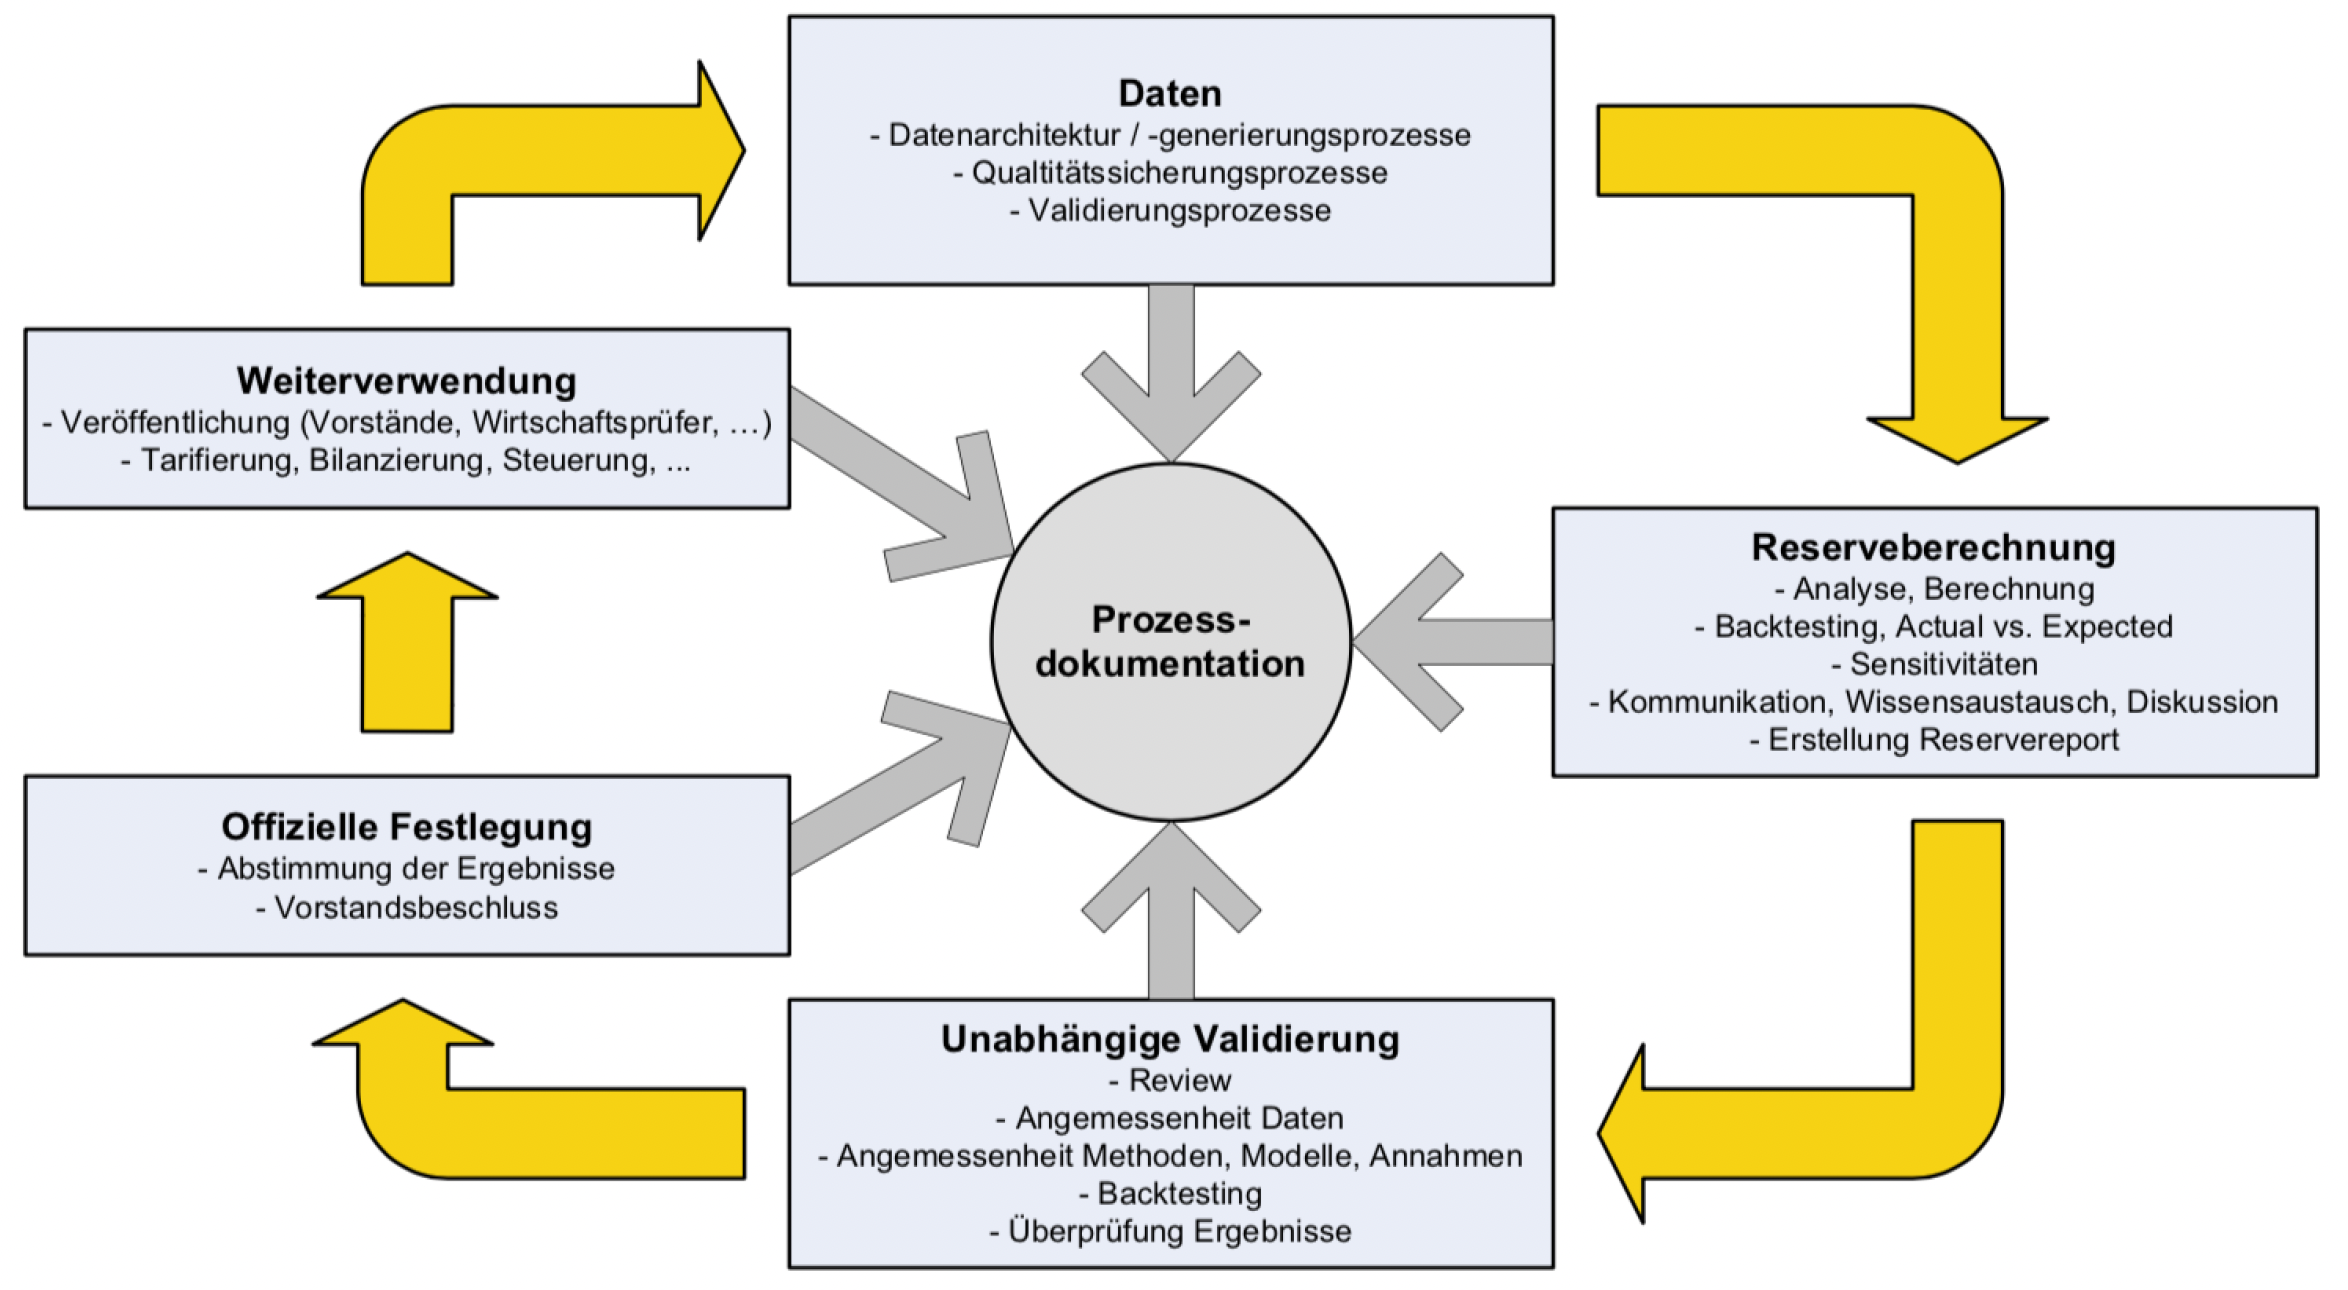
\includegraphics[width=\textwidth]{Bilder/Reservierungsprozess.png}
\end{figure}


\subsubsection{Allgemeine Aspekte}
\begin{itemize}
	\item Umfang und Turnus
	\item Rollenbeschreibung der Beteiligten
	\item Organisationsstruktur
	\item Unabh\"angigkeit und Objektivit\"at
	\item Interne Kontrollen
\end{itemize}

\subsubsection{Daten}
\begin{itemize}
	\item Transparanz, Nachvollziehbarkeit der Datengenerierung
	\item Dokumentation des Prozesses
	\item Beschreibung Datenarchitektur
	\item unternehmensweite Konsisntenz
	\item ausreichende Datenhistorie
	\item Qualit\"atssicherung mit angemessener Dokumentation
	\item automatische und manuelle Tests
	\item Plausibilisierung
\end{itemize}

\subsubsection{Reserveberechnung}
\begin{itemize}
	\item Festlegung von Umfang der Analysen und Konsistenz zu SII
	\item Welche Software?
	\item Welche Annahmen werden wie getroffen?
	\item Wie sieht die aktuarielle Entscheidungsfindung aus und ist diese transparent dokumentiert?
	\item Wie wird kontrolliert und validiert?
\end{itemize}

\subsubsection{Unabh\"angige Validierung}
\begin{itemize}
	\item insb. durch SII gefordert
	\item \"Uberpr\"ufung der Angemessenheit der Daten, Modelle, Methoden, Annahmen und Ergebnisse
	\item Backtesting
	\item unabh\"angig von der Berechnung
\end{itemize}

\subsubsection{Prozessdokumentation}
\begin{itemize}
	\item Prozessbeschreibung
		\begin{itemize}
			\item �berblick
			\item Schnittstellen
			\item Prozessgestaltung
			\item Ausf\"uhrung
			\item Versionshistorie
			\item Kontrollsystem
			\item Tests
			\item Dokumentationsrichtlinien
		\end{itemize}
	\item Dokumentation der Kontrollprozesse
\end{itemize}

\subsection{Zweck und Aufbau des Reserveberichts}
\begin{itemize}
	\item Reservebericht 
	\begin{itemize} 
		\item individuell an Umfang und Verwendungszweck angepasst
		\item an Zielgruppen orientiert
		\item als Basis der VmF zur Erf�llung ihrer Pflichten
	\end{itemize}
	\item Inhalte des Reserveberichts
	\begin{itemize}
		\item Zweck der Reserveanalyse, Auftraggeber
		\item Umfang der Reserveanalyse
		\item Relevante Entwicklungen und wesentliche Kennzahlen
		\item Daten und Methoden
		\item Zusammenfassung der Ergebnisse
		\item Vergleich mit Vorperioden
	\end{itemize}
\end{itemize}

\chapter{Versicherungstechnische R�ckstellungen in der Rechnungslegung}

\section{IFRS 17, HGB, SII im Vergleich}

Unterschieden wird nach:
\begin{itemize}
	\item IFRS 17: entscheidungsn\"utzliche Informationen bzgl. Verm\"ogens- und Finanzlage
	\item HGB: Informationsvermittlung und Aussch\"uttungsbemessung
	\item SII: Bestimmung der Eigenmittel als Verlustdeckungspotenzial 
\end{itemize}

\subsection{Versicherungsvertr\"age}

\begin{itemize}
	\item IFRS 17: Vertr\"age, die signifikantes Versicherungsrisiko \"ubertragen (Versicherungsrisiko wird von Finanzrisiko abgegrenzt)
	\item HGB: keine eigene Definition von Versicherungsvertr\"agen, aber Anforderungen an den Risikotransfer von R\"uckversicherung
	\item SII: keine eigene Definition von Versicherungsvertr\"agen und R\"uckversicherungsvertr\"agen
\end{itemize}

\subsection{Kosten als Teil der vers.techn. R\"uckstellungen}

\begin{itemize}
	\item IFRS 17: SRK und Verwaltungskosten werden einbezogen, Ber\"ucksichtigung der variablen Abschlusskosten bei CSM, keine allgemeine Verwaltungskosten ber\"ucksichtigt
	\item HGB: SRK einbezogen, keine allgemeine Verwaltungskosten ber\"ucksichtigt
	\item SII: SRK, Vertragsverwaltungskosten, Abschlusskosten, Kosten der Verwaltung der Kapitalanlagen einbezogen
\end{itemize}

\subsection{Datenqualit\"at}
\begin{itemize}
	\item HGB: Grunds�tze ordnungsgem\"a{\ss}er Buchf\"uhrung
	\item SII:
	\begin{itemize}
		\item Vollst�ndigkeit, Richtigkeit und Angemessenheit gefordert
		\item bezieht sich auf interne und externe Daten
		\item Angemessenheit muss nachweisbar sein, daf\"ur umfangreiche Dokumentation erforderlich
	\end{itemize}
	\item IFRS 17: kein eigener Abschnitt zur Datenqualit\"at
\end{itemize}

\section{Bewertungsmodell unter IFRS 17}

Building Block Approach (u.U. Premium Allocation Approach zugelassen):
\begin{itemize}
	\item Basis sind die erwarteten Zahlungsstr�me
	\item Diskontierung
	\item Risikomarge zur Deckung der Unsicherheiten (keine Berechnungsvorgabe, aber geforderte Eigenschaften)
	\item Servicemarge (CSM) dient der Neutralisierung von Gewinnen bei Vertragsabschluss. Bei LIC (Liability for incurred claims keine CSM)
	\item LRC (Liability for remaining coverage) f�r bound but not incepted onerous contracts wird eine Drohverlustr\"uckstellung (Loss Component) gebildet, f\"ur incepted contracts eine CSM
\end{itemize}

\section{Bewertungsmodell unter HGB}
Retrospektive Bewertung der Beitr\"age mit prospektiver Bildung von R"uckstellungen f\"ur drohende Verluste. Bewertung der Schadenr\"uckstellung prospektiv:
\begin{itemize}
	\item Einzelbewertung f\"ur bekannte Versicherungsf\"alle
	\item Gruppenbewertung f\"ur unbekannte Sp\"atsch\"aden
	\item Rentenverbindlichkeiten separat bewerten
	\item Zus\"atzliche Schwankungsr\"uckstellungen zur Stabilisierung
\end{itemize}

\subsection{Schwankungsr\"uckstellungen unter HGB}
	\begin{itemize}
		\item zu bilden, wenn erhebliche Schwankungen erwartet werden oder Schwankungen nicht durch Beitr\"age ausgeglichen werden k\"onnen oder durch R\"uckversicherung gedeckt sind
		\item Nur bei Schaden/Unfall
		\item Ermittlung und Bildung f\"ur jeden Versicherungszweig separat.
		\item Berechnung Standardfall:
		\begin{itemize}
			\item $\{1,...,n\}$ der Beobachtungszeitraum vor Bilanzjahr $n+1$
			\item $\bar{q}$ die durchschnittliche Schadenquote, $\bar{\sigma} = \sqrt{\frac{1}{n-1}\sum^{n}_{i=1}(q_i-\bar{q})^2}$ die Standardabweichung
			\item Sollbetrag $SB=4,5 \cdot \bar{\sigma} \cdot P$, $P \hat{=}$ verdiente Beitr\"age des Bilanzjahres
			\item[(1)] $SR^{(1)}_{n+1} = \begin{cases}
				min(SR_n + 3,5\% \cdot SB; SB) & \text{falls } SR_n \leq SB \\
				SR_n & \text{sonst}
			\end{cases}$ 
			\item $B=(\bar{q} - q_{n+1}) \cdot P$ ,\ ($\bar{q} > q_{n+1} \rightarrow$ B Unterschaden, $\bar{q} < q_{n+1} \rightarrow$ -B \"Uberschaden)
			\item[(2)] Erh\"ohung bei Unterschaden: \\ $SR^{(2)}_{n+1} = \begin{cases}
				min(SR_{n+1}^{(1)} + B; SB) & \text{falls } SR_{n+1}^{(1)} \leq SB \text{ und } \bar{q} > q_{n+1}\\
				SR_n	{(1)} & \text{sonst}
			\end{cases}$  
			\item[(3)] Entnahme des \"Uberschadens: \\
			$SR^{(3)}_{n+1} = \begin{cases}
				max(SR_{n+1}^{(2)} + B; 0) & \text{falls } \bar{q} < q_{n+1}\\
				SR_{n+1}^{(2)} & \text{sonst}
			\end{cases}$ 
			\item[(4)] Begrenzung durch Sollbetrag sicherstellen \\
			$SR_{n+1} = min(SR_{n+1}^{(3)}; SB)$
			\item Schadenquote nach Schwankung: $q_{n+1}^{nS} = q_{n+1} + \frac{SR_{n+1} - SR_n}{P}$
			\item Falls $SR_{n+1} = SR_n + 3,5\% \cdot SB + B$, dann $q_{n+1}^{nS} = \bar{q} + 3,5\% \cdot 4,5 \cdot \bar{\sigma}$
		\end{itemize}
			
	\end{itemize}

\subsection{Bewertungsmodell unter SII}

\begin{itemize}
	\item prospektive Bewertung des gesamten Versicherungsvertrags:
	\begin{itemize}
		\item Basis: erwartete Zahlungsstr\"ome
		\item risikolose Diskontierung
		\item Risikomarge
	\end{itemize}
	\item vers.techn. R\"uckstellungen (TPs) beinhalten Claims Provisions, Premium Provisions (beides diskontiert) und Risikomarge
	\item BE einer vers.techn. R\"uckstellung $\hat{=}$ wahrscheinlichkeitsgewichteter Durchschnitt zuk\"unftiger Zahlungensstr\"ome unter Ber\"ucksichtigung des Zeitwerts des Geldes (Barwert) und unter Verwendung einer risikofreien Zinskurve (existiert brutto und netto) 
\end{itemize}

\subsection{Schadenr\"uckstellungen unter SII}

\begin{itemize}
	\item Schadenr\"uckstellungen decken die Verpflichtungen aus bereits eingetretenen Sch\"aden zu Vertr\"agen, die vor dem Bilanzstuchtag bestanden haben inkl. noch unbekannter Rentenf\"alle
	\item BE einer Schadenr\"uckstellung $\hat{=}$ diskontierter wahrscheinlichkeitsgewichteter Durchschnitt k�nftiger Sch\"aden, die sich vor dem Bilanzstichtag ereignet haben
	\item Zuk\"unftige Zahlungsstr\"ome der SRK sind Teil der Schadenr\"uckstellungen
\end{itemize}

\subsection{Pr\"amienr\"uckstellungen unter SII}

\begin{itemize}
	\item Pr\"amienr\"uckstellungen $\hat{=}$ Saldo aus Barwert der Verpflichtungen und Barwert zuk\"unftiger Pr\"amien
	\item Barwert der Verpflichtungen bezieht sich auf zuk\"unftig eintretende Schadenf\"alle aus Vertr\"agen, die zum Bilanzstichtag bestanden haben
\end{itemize}

\subsubsection{Ansatz von Versicherungsvertr\"agen unter SII}
\begin{itemize}
	\item Bei Berechnung der Pr\"amienr\"uckstellungen sind alle Zahlungsstr\"ome zu ber\"ucksichtigen
	\item Entscheidend ist ob Beginn des Versicherungsschutzes oder der Vertragsabschluss vor Bilanzstichtag liegt
\end{itemize}

\subsubsection{Vertragsgrenzen unter SII}
\begin{itemize}
	\item Anzusetzende Vertr\"age sind bis zum folgenden Zeitpunkt in der Berechnung der Pr\"amienr\"uckstellungen zu ber\"ucksichtigen:
	\begin{itemize}
		\item bis zu dem Tag, an dem das Versicherungsunternehmen das einseitige Recht hat, den Vertrag zu beenden
		\item bis zu dem Tag, an dem das Versicherungsunternehmen das einseitige Recht hat, die Pr\"amienh\"ohe oder den Leistungsumfang anzupassen
	\end{itemize}	
\end{itemize}

\subsubsection{Vereinfachtes Berechnungsverfahren zur Sch\"atzung der Pr\"amienr\"uckstellung}

\begin{itemize}
	\item undiskontierte Pr\"amienr\"ucktellungen \begin{equation}
		BE_{premium} = (CR - AER) \cdot VM + (CR - 1) \cdot FP
	\end{equation} 
	\item CR: gesch\"atzte, undiskontierte Schaden-Kosten-Quote
	\item AER: gesch\"atzte Abschlusskostenqote f\"ur Abschlusskosten des aktuellen Bestandes, die bis zum Laufzeitende angefallen sind
	\item VM: \"okonomische Beitrags\"ubertr\"age aus bereits bekannten Vertr\"agen
	\item FP: gesch\"atzte, zuk\"unftige, undiskontierte Brutto-Pr\"amie f\"ur alle Vertr\"age des aktuellen Bestandes, die gem\"a{\ss} der Grenzen der Versicherungsvertr\"age zu ber\"ucksichtigen sind
 \end{itemize}

\subsection{R\"uckversicherung unter SII}

\begin{itemize}
	\item BE Brutto - Einforderbare Betr\"age aus RV = BE Netto
	\item Einforderbare Betr\"age getrennt nach Pr\"amien- und Schadenr\"uckstellungen (und anerkannte Renten)
	\item Segmentierung in homogene Risikogruppen
	\item Unterschiedliche Formen der RV (proportional, nicht-proportional, Stop-Loss, fakultativ)
	\item Wiederauff\"ullungspr\"amien ber\"ucksichtigen
	\item M\"oglichen Ausfall der RV einkalkulieren
	\item Einforderbare Betr\"age aus RV beim Erstversicherer = versicherungstechnische R\"uckstellungen beim RV
\end{itemize}

\subsection{Risikomarge unter SII}
\begin{itemize}
	\item stellt sicher, dass der Wert der vers.techn. R\"uckstellungen dem Betrag entspricht, den VU fordern fordern w\"urden, um die Versicherungsverpflichtungen \"ubernehmen und erf\"ullen zu k�nnen
	\item  $RM = CoC \cdot \sum_{t\geq 0} \frac{SCR_{RU}(t)}{(1+r_{t+1})^{t+1}}$
	\item $CoC$ = Kapitalkostensatz (6\%)
	\item $SCR_{RU}(t)$: Solvenzkapitalanforderung des Referenzunternehmens \textit{RU} nacht \textit{t} Jahren
	\item $r_{t+1}$: risikofreier Zins zur Laufzeit $t+1$
\end{itemize}

\section{Grundlagen der aktuariellen Schadenreservebewertung}

\subsection{Grundlagen und Bezeichnungen}

\subsubsection{Abwicklungsdreieck bzw. -rechteck}

\begin{figure}[H]
\centering
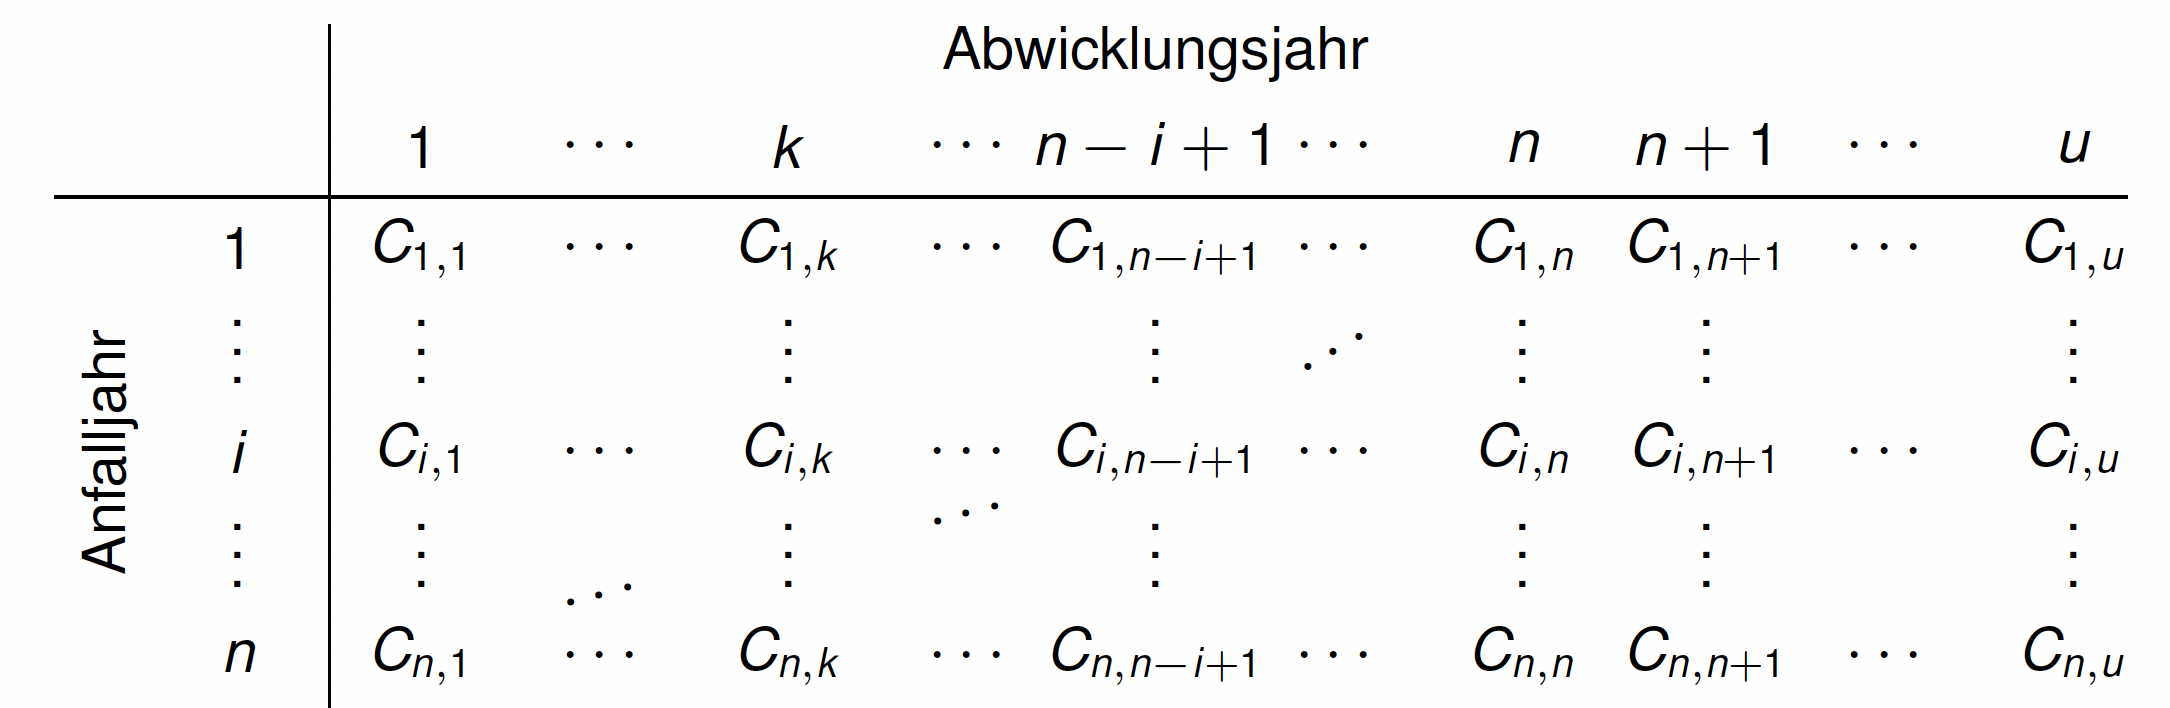
\includegraphics[width=\textwidth]{Bilder/Abwicklungseck.png}
\end{figure}

\begin{itemize}
	\item $C_{i,k}$ kumulativer Stand des AJs \textit{it} nach \textit{k} Abwicklungsjahren
	\item $1 \leq i \leq n$ und $1 \leq k \leq u$
	\item $n<u$: Nachlauf/Tail
	\item Zeilen k\"onnen sein: Anfalljahre, Zeichnungsjahre, Meldejahre
	\item Abwicklungsjahre
	\begin{itemize}
		\item Zedentensichtweise: RV definiert das Abwicklungsjahr, in dem das abgerechnete Quartal des Zedenten liegt
		\item Finanzsichtweise: Basis f\"ur Abwicklungsjahr ist das Jahr, in dem die Abrechnung beim RV verbucht wurde
	\end{itemize}
	\item Segmentierung konsistent zur Tarifierung halten
	\item $S_{i,k} = C_{i,k} - C_{i,k-1}$
	\item $R_i = C_{i,u} - C_{i,n-i+1} = S_{i,n-i+2} + ... + S_{i,u}$
	\item $R = R_1 + ... + R_n$
	\item IBNR = IBNYR + IBNER (incurred but not yet reported + incurred but not enough reserved)
	\item Kernproblem: Bestimmung einer Sch\"�tzung $\hat{R}_i$ f\"ur $R_i$ bzw. $E(R_i)$
	\item Anfalljahre unabh�ngig voneinander (problematisch, da Inflation z.B. kein Anfalljahreseffekt ist)
	\item Bereinigung von Gro{\ss}sch\"aden und Inflation u.U. notwendig
	\item Manche Projektionsverfahren verwenden ein Volumen- bzw. Exposurema{\ss} $v_i$ f\"ur das AJ \textit{i}
\end{itemize}

\subsection{Segmentierung}

\begin{itemize}
	\item Einteilung eines Bestandes in hinreichend gro{\ss}e, aber m\"oglichst homogene Risikogruppen bzw. Einteilung von Sch\"aden in Gruppen anhand von Schadenmerkmalen
	\item Muss zu Anforderungen der externen Rechtslegung passen:
	\begin{itemize}
		\item HGB: Unterteilung in Unfall, Kranken, KFZ-Haftpflicht, KFZ-Sonstige, Transport und Luftfahrt, Feuer und Sach, Haftpflicht, Kredit und Kaution, Rechtsschutz, Beistandsleistungen, Sonstige
		\item IFRS: Keine Anforderungen
		\item SII: Homogene Risikogruppen, mindestens nach SII LoBs
	\end{itemize}
\end{itemize}


\subsection{Sich \"andernde Rahmenbedingungen - Inflation}

\subsubsection{interne Rahmenbedingungen}
\begin{itemize}
	\item Schadenregulierung
	\item Praxis der Einzelfallreservierung
	\item Bestandszusammensetzung
	\item Tarifbedingungen
	\item Beitragsanpassungen
	\item Datenverarbeitung
	\item [$\rightarrow$] ber\"ucksichtigen und Datenhistorie anpassen
\end{itemize}

\subsubsection{externe Rahnenbedingungen}

\begin{itemize}
	\item Gesetzlicher Rahmen, Recht, Steuern
	\item Gesellschaftliche, soziale, demographische, politische Rahmenbedingungen
	\item Medizinischer Fortschritt, steigende Lebenserwartung
	\item Technologischer Fortschritt
	\item \"Okologische Entwicklungen
	\item \"okonomische Rahmenbedingunen (z.B. Inflation)
	\item [$\rightarrow$] individuelle Ber\"ucksichtigung, z.B. Inflationsanpassung $S_{i,k}^{I}=\frac{I_n}{I_{i+k-1}} \cdot S_{i,k}$
	\item [$\rightarrow$] zuk\"unftige Zahlungsstr\"ome $\widehat{S_{i,k}} = \frac{I_{i+k-1}}{I_n} \cdot \widehat{S_{i,k}^I}$ (Inflationierung der Zukunft)
	\item Praxis: Daten nicht bereinigt, Inflation implizit ber\"ucksichtigt und bei Bedarf Superimposed Inflation on top
\end{itemize}

\subsection{Raten\"anderungen, Pr\"amienzyklen und Reservezyklen}

\begin{itemize}
	\item J\"ahrliche Anpassung der Pr\"amie m\"oglich
	\item Raten\"anderung: h\"ohere oder niedrigere Pr\"amien f\"ur gleiche Risiken
	\item Praxis: Messung schwierig, da oft Tarife auch leicht modifiziert werden. Ratenverbesserungen, wenn die Pr\"amie steigt und das Risiko gleich bleibt
	\item Pr\"amienzyklus: einige Jahre Ratenverbesserungen, dann Ratenverschlechterungen (harter und weicher Markt)
	\begin{itemize}
		\item nicht ausk\"ommliche Pr\"amien f\"uhren zu Preiserh\"ohungen
		\item ausk\"ommliche zu Gewinnen und erlauben damit Ratenverschlechterungen 
		\item solche Zyklen auch bei Reserven zu beobachten (Reserveerh\"ohung oder -aufl\"osung
	\end{itemize}
\end{itemize}

\subsection{Die Behandlung von Ausrei{\ss}ern, Gro{\ss}- und Kumulsch\"aden}

\begin{itemize}
	\item Ausrei{\ss}er: 
	\begin{itemize}	
		\item deutlich anderes Abwicklungsverhalten
		\item Anteil gro{\ss} genug, um relevant zu sein
		\item z.B. Gro{\ss}- oder Kumulsch\"aden
	\end{itemize}
	\item Gro{\ss}schadengrenze muss festgelegt werden
	\begin{itemize}
		\item Quantil der Schadenh\"ohenverteilung
		\item Prozentsatz des erwarteten Endschadenstands des Anfalljahres
		\item Fest gew\"ahlter Betrag als Grenze
	\end{itemize}
	\item Separation der Gro{\ss}- und Kumulsch\"aden
		\begin{itemize}
			\item Separation aus Abwicklungsdaten
			\item Problem: vorhandene Sch\"aden, die sp\"ater gro{\ss} werden, werden inkonsistent behandelt
			\item Kappung an Gro{\ss}schadengrenze
			\item Problem: Erzeugt k\"unstliches Abwicklungsverhalten
			\item Gl\"attung des Abwicklungsdreiecks
			\item Problem: Was sind objektive Kriterien zur Umverteilung?
		\end{itemize}
	\item Gro{\ss}sch\"aden werden separat in Gro{\ss}schadendreick oder \"uber Einzelbewertung betrachtet
	\item R\"uckstellungen f\"ur zuk\"unftige Gro{\ss}sch\"aden
\end{itemize}

\subsection{Abwicklungsmuster und Methoden der Reservebewertung}

\begin{figure}[H]
\centering
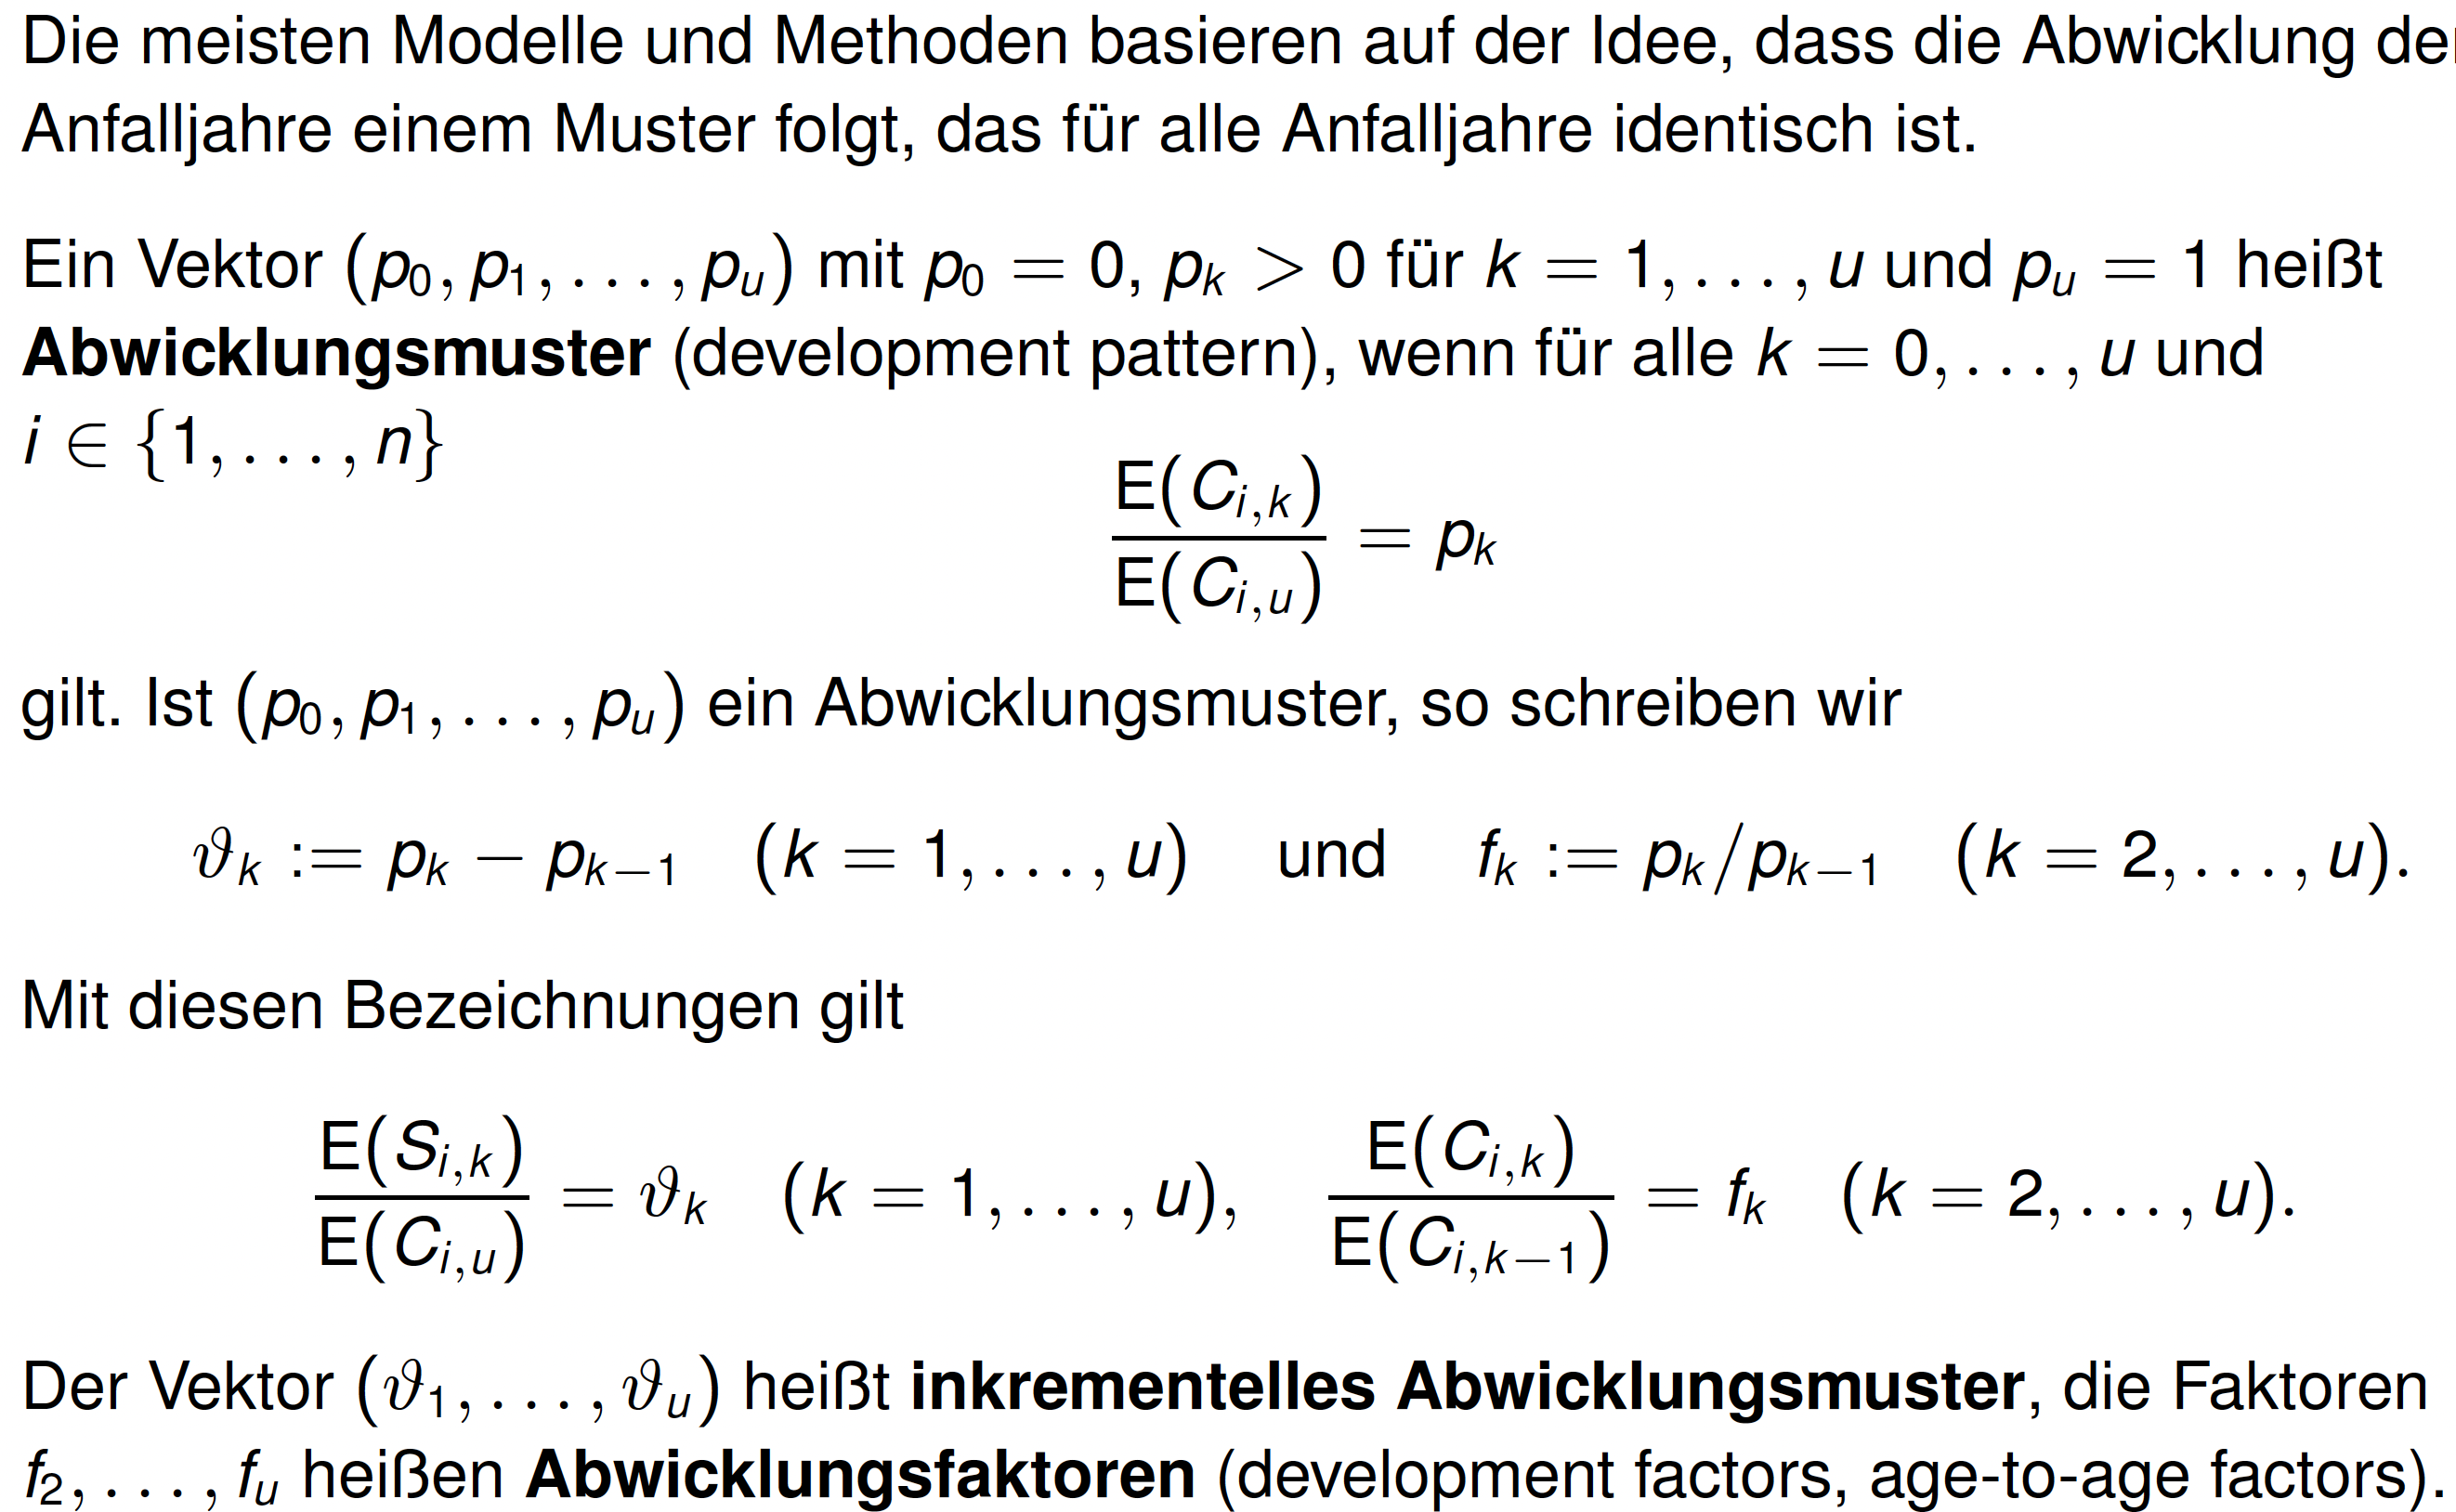
\includegraphics[width=\textwidth]{Bilder/Abwicklungsmuster1.png}
\end{figure}

\begin{figure}[H]
\centering
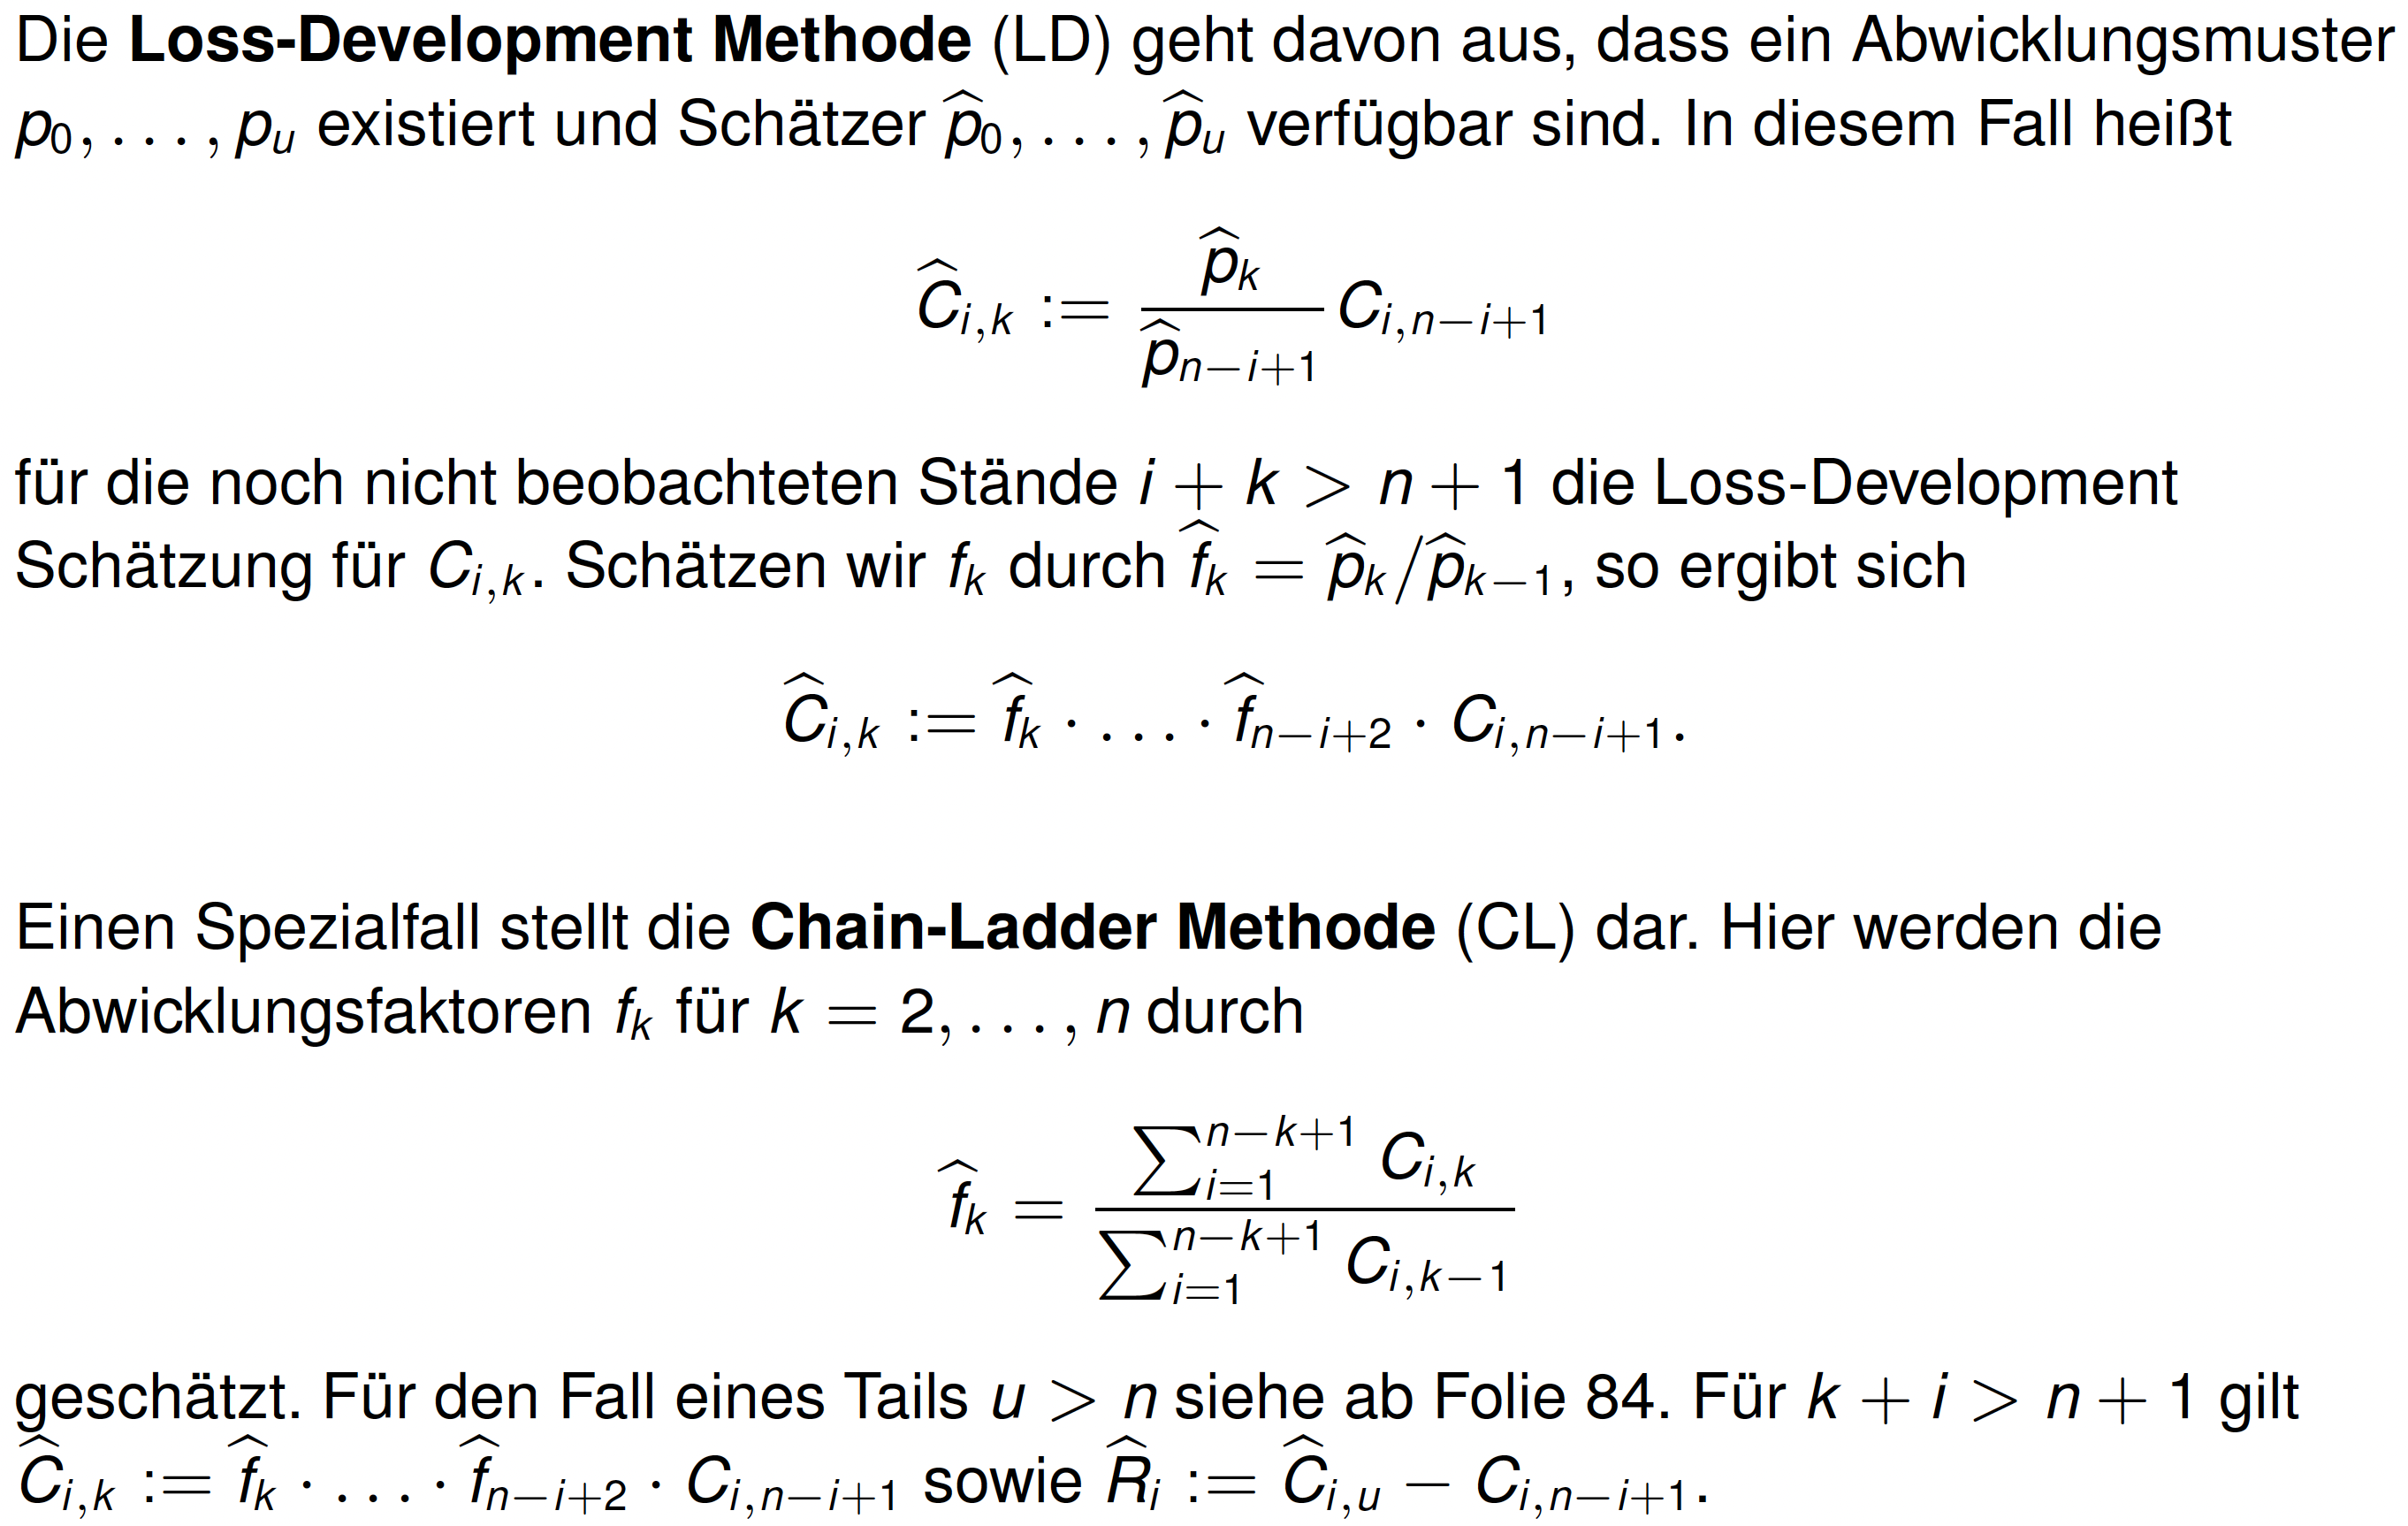
\includegraphics[width=\textwidth]{Bilder/Abwicklungsmuster2.png}
\end{figure}

\begin{figure}[H]
\centering
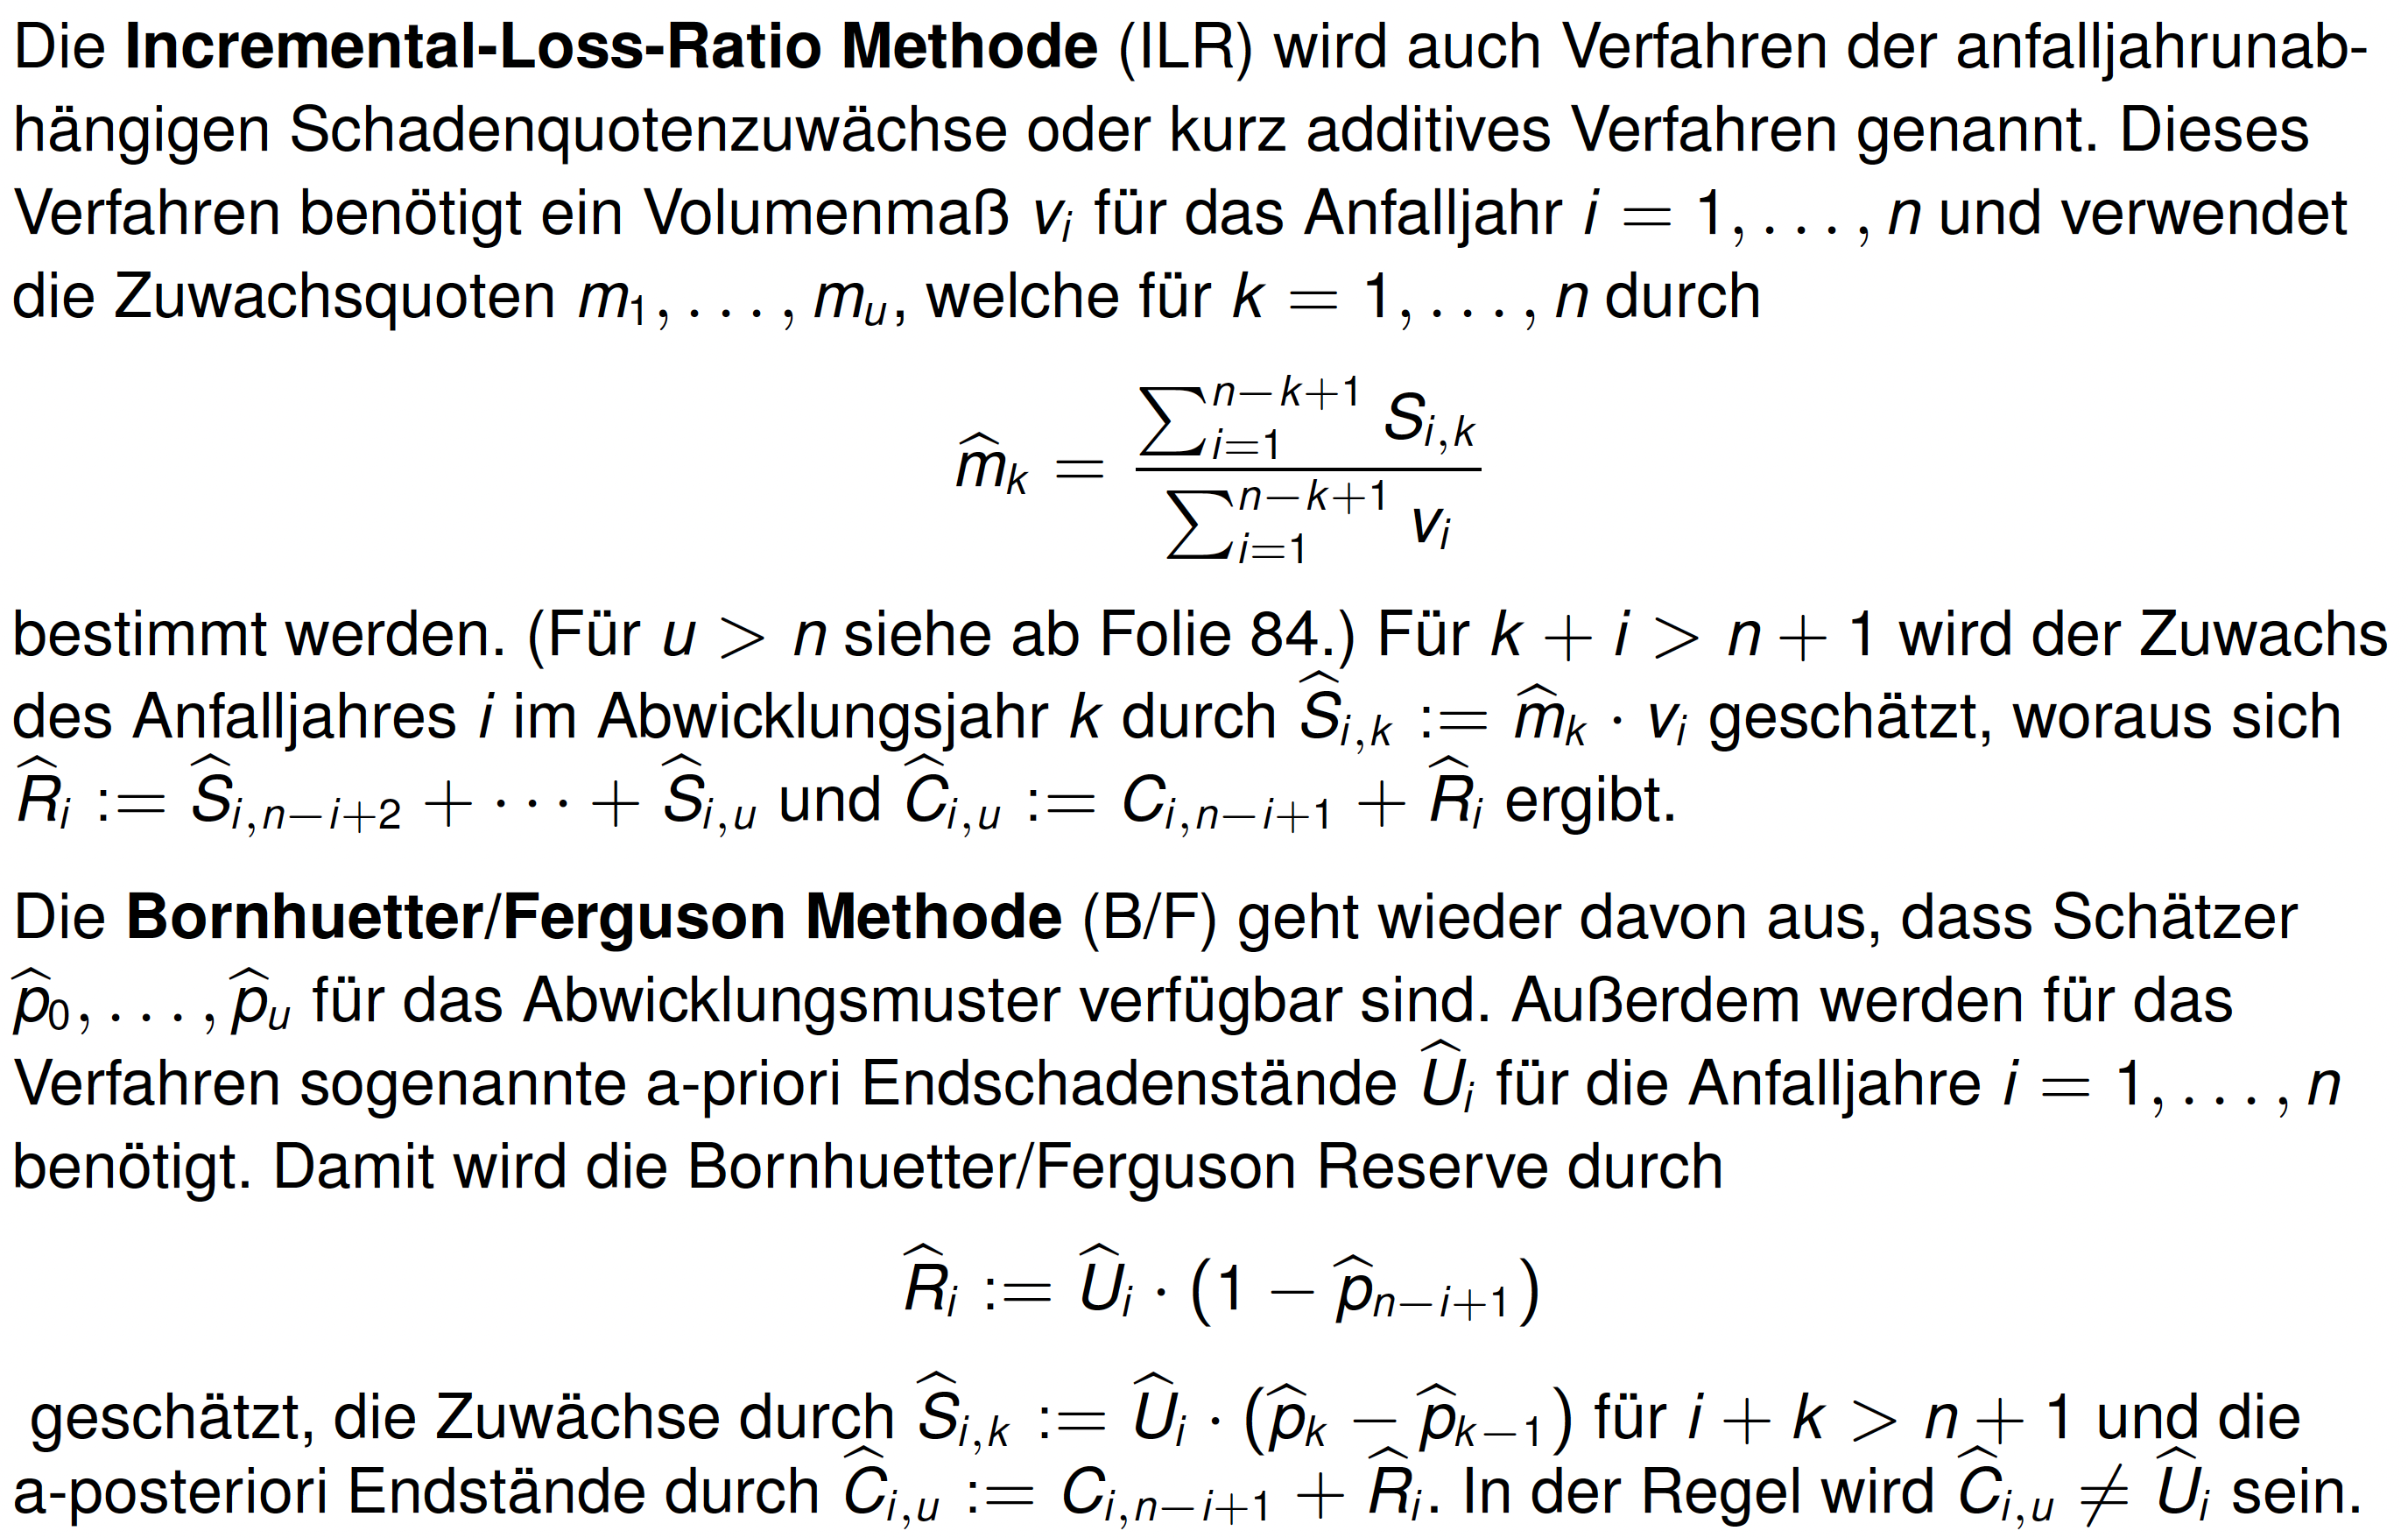
\includegraphics[width=\textwidth]{Bilder/Abwicklungsmuster3.png}
\end{figure}

\begin{figure}[H]
\centering
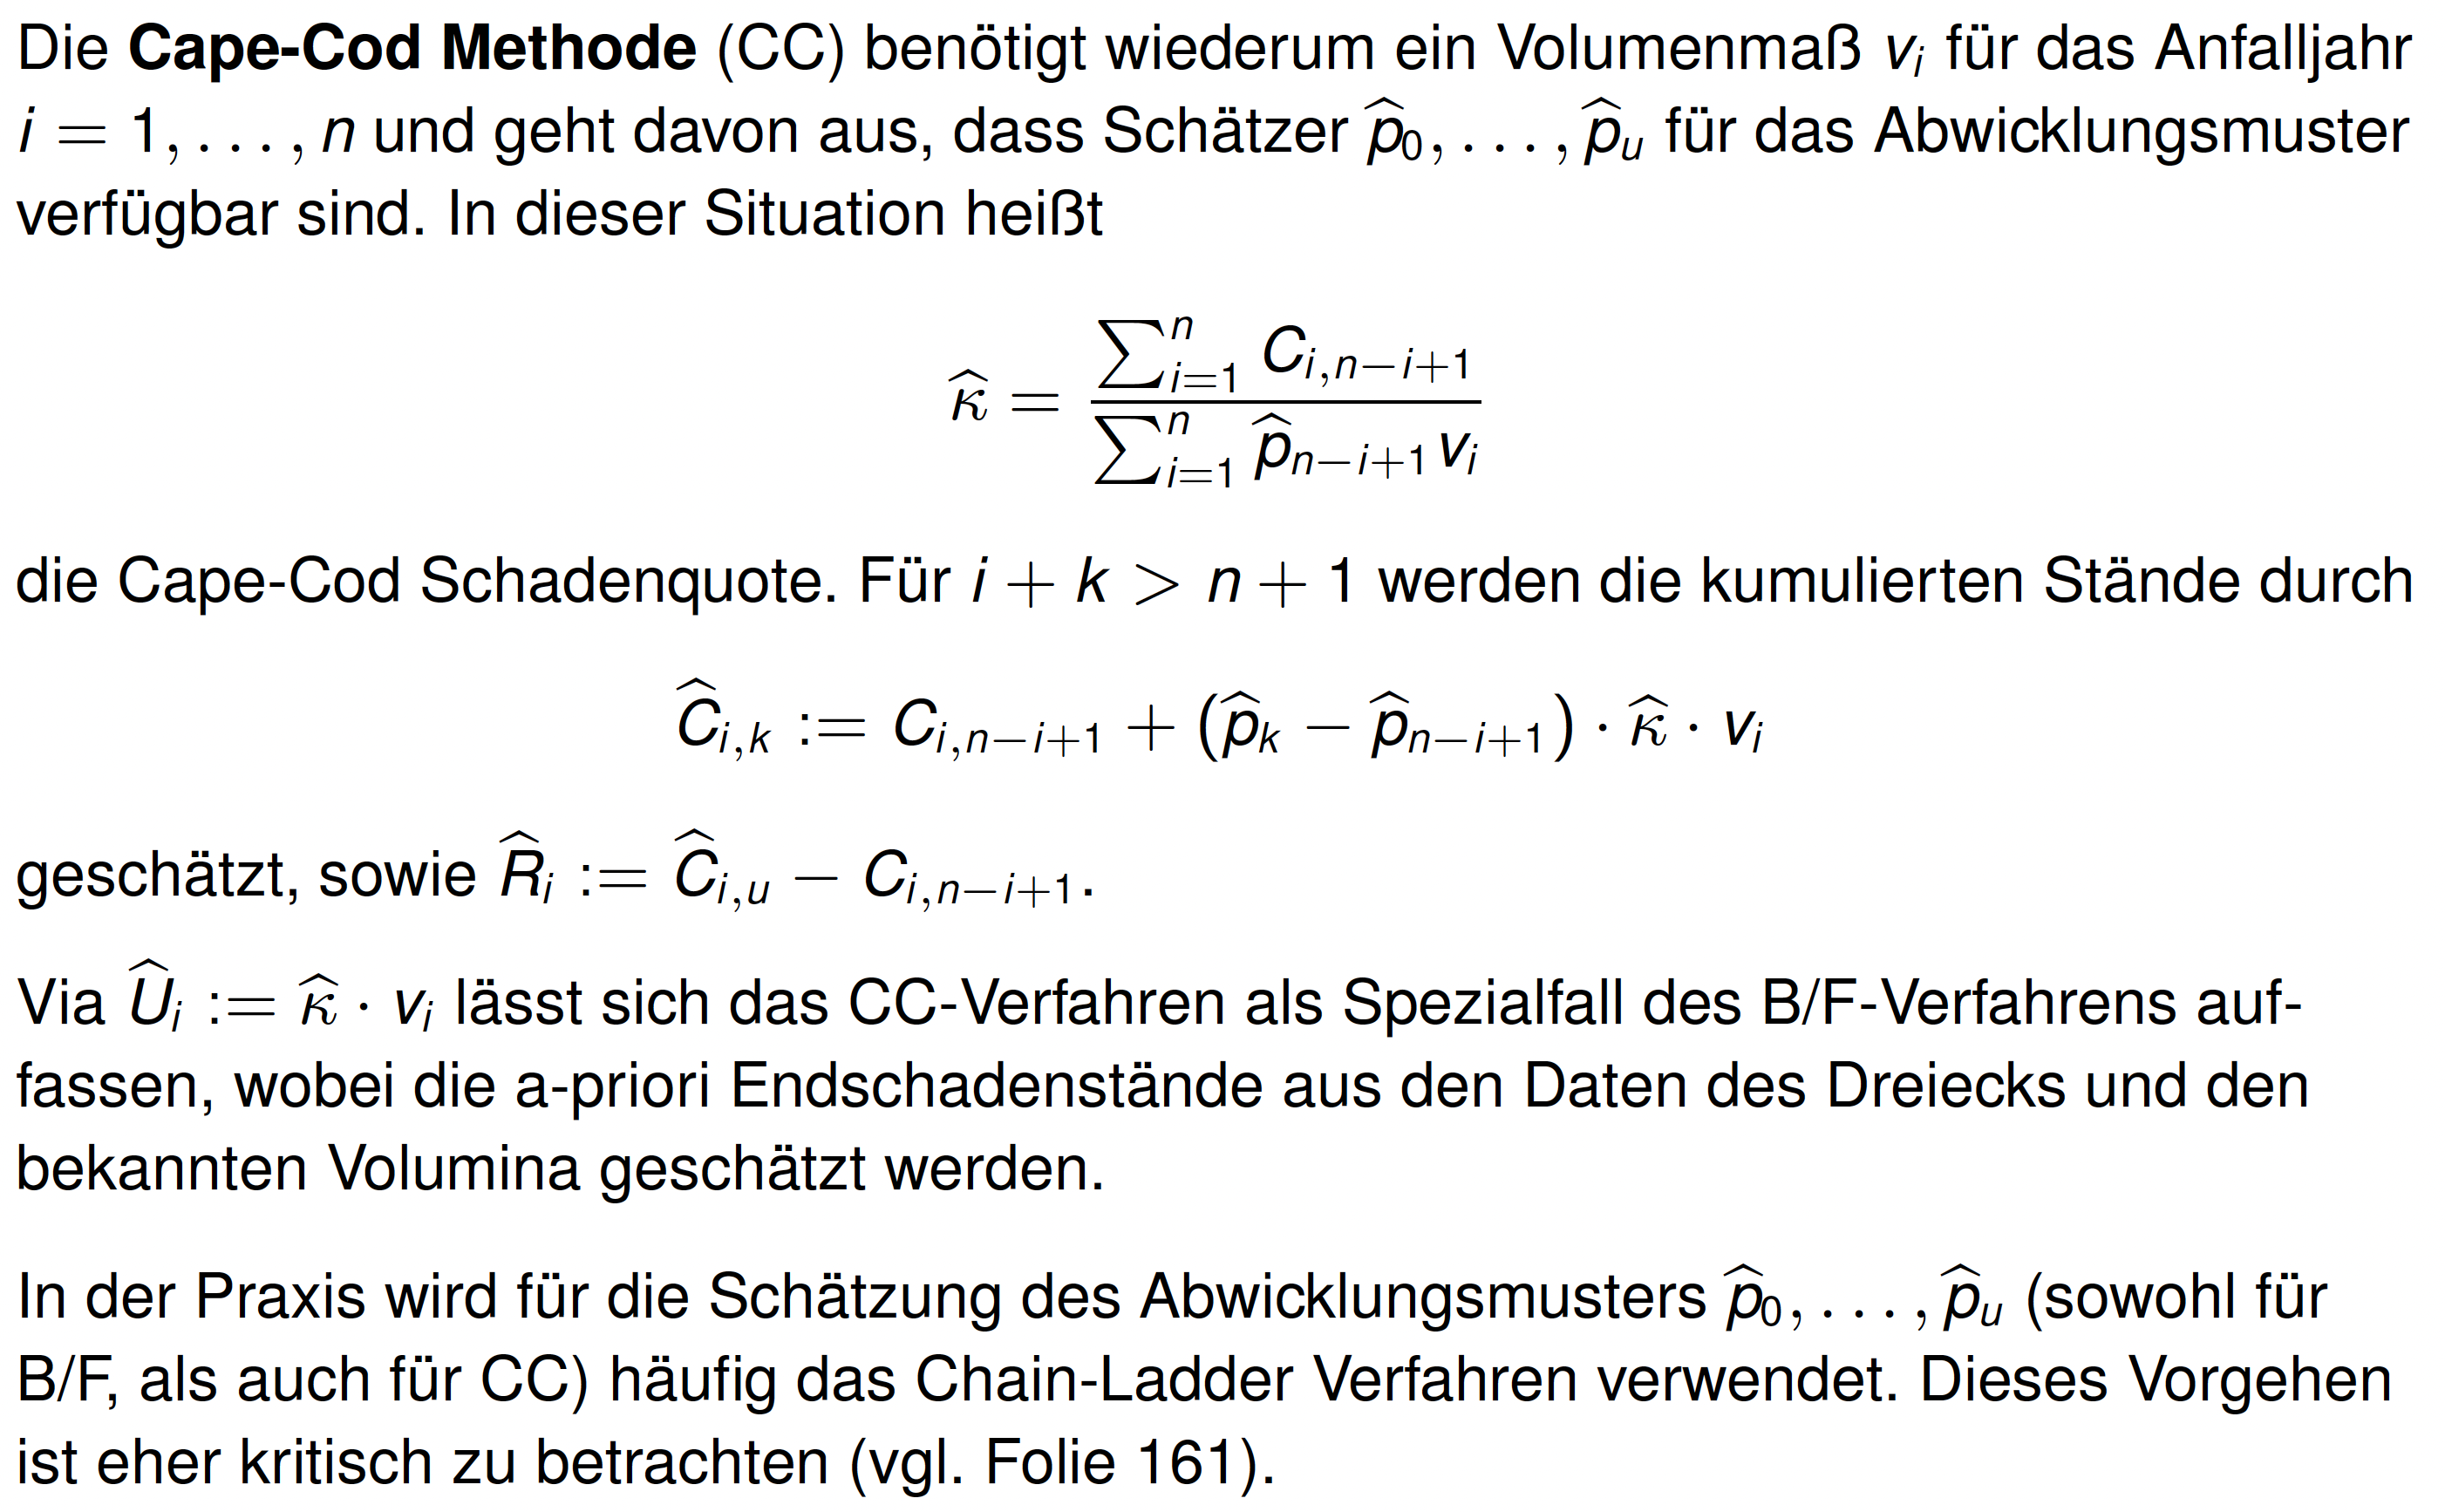
\includegraphics[width=\textwidth]{Bilder/Abwicklungsmuster4.png}
\end{figure}

\subsection{Behandlung Nachlauf und Gl\"attung}

\begin{itemize}
	\item meist bei lang-abwickelnden Sparten, wie z.B. Haftpflicht
	\item Abwicklungsmuster unterstellen: $f_k = \frac{E(C_{i,k})}{E(C_{i,k-1})}$ f\"ur $k=n+1,...,u$
	\item Zahlung: monoton fallende Faktoren, die sich der 1 n\"ahern
	\item Aufw\"ande: Faktoren zwischen 0 und 1 m\"oglich
	\item Sch\"atzung der Faktoren mit Abwicklungsfunktion $\phi:\mathbb{N} \rightarrow \mathbb{R}_+:$
\end{itemize}

\begin{figure}[H]
\centering
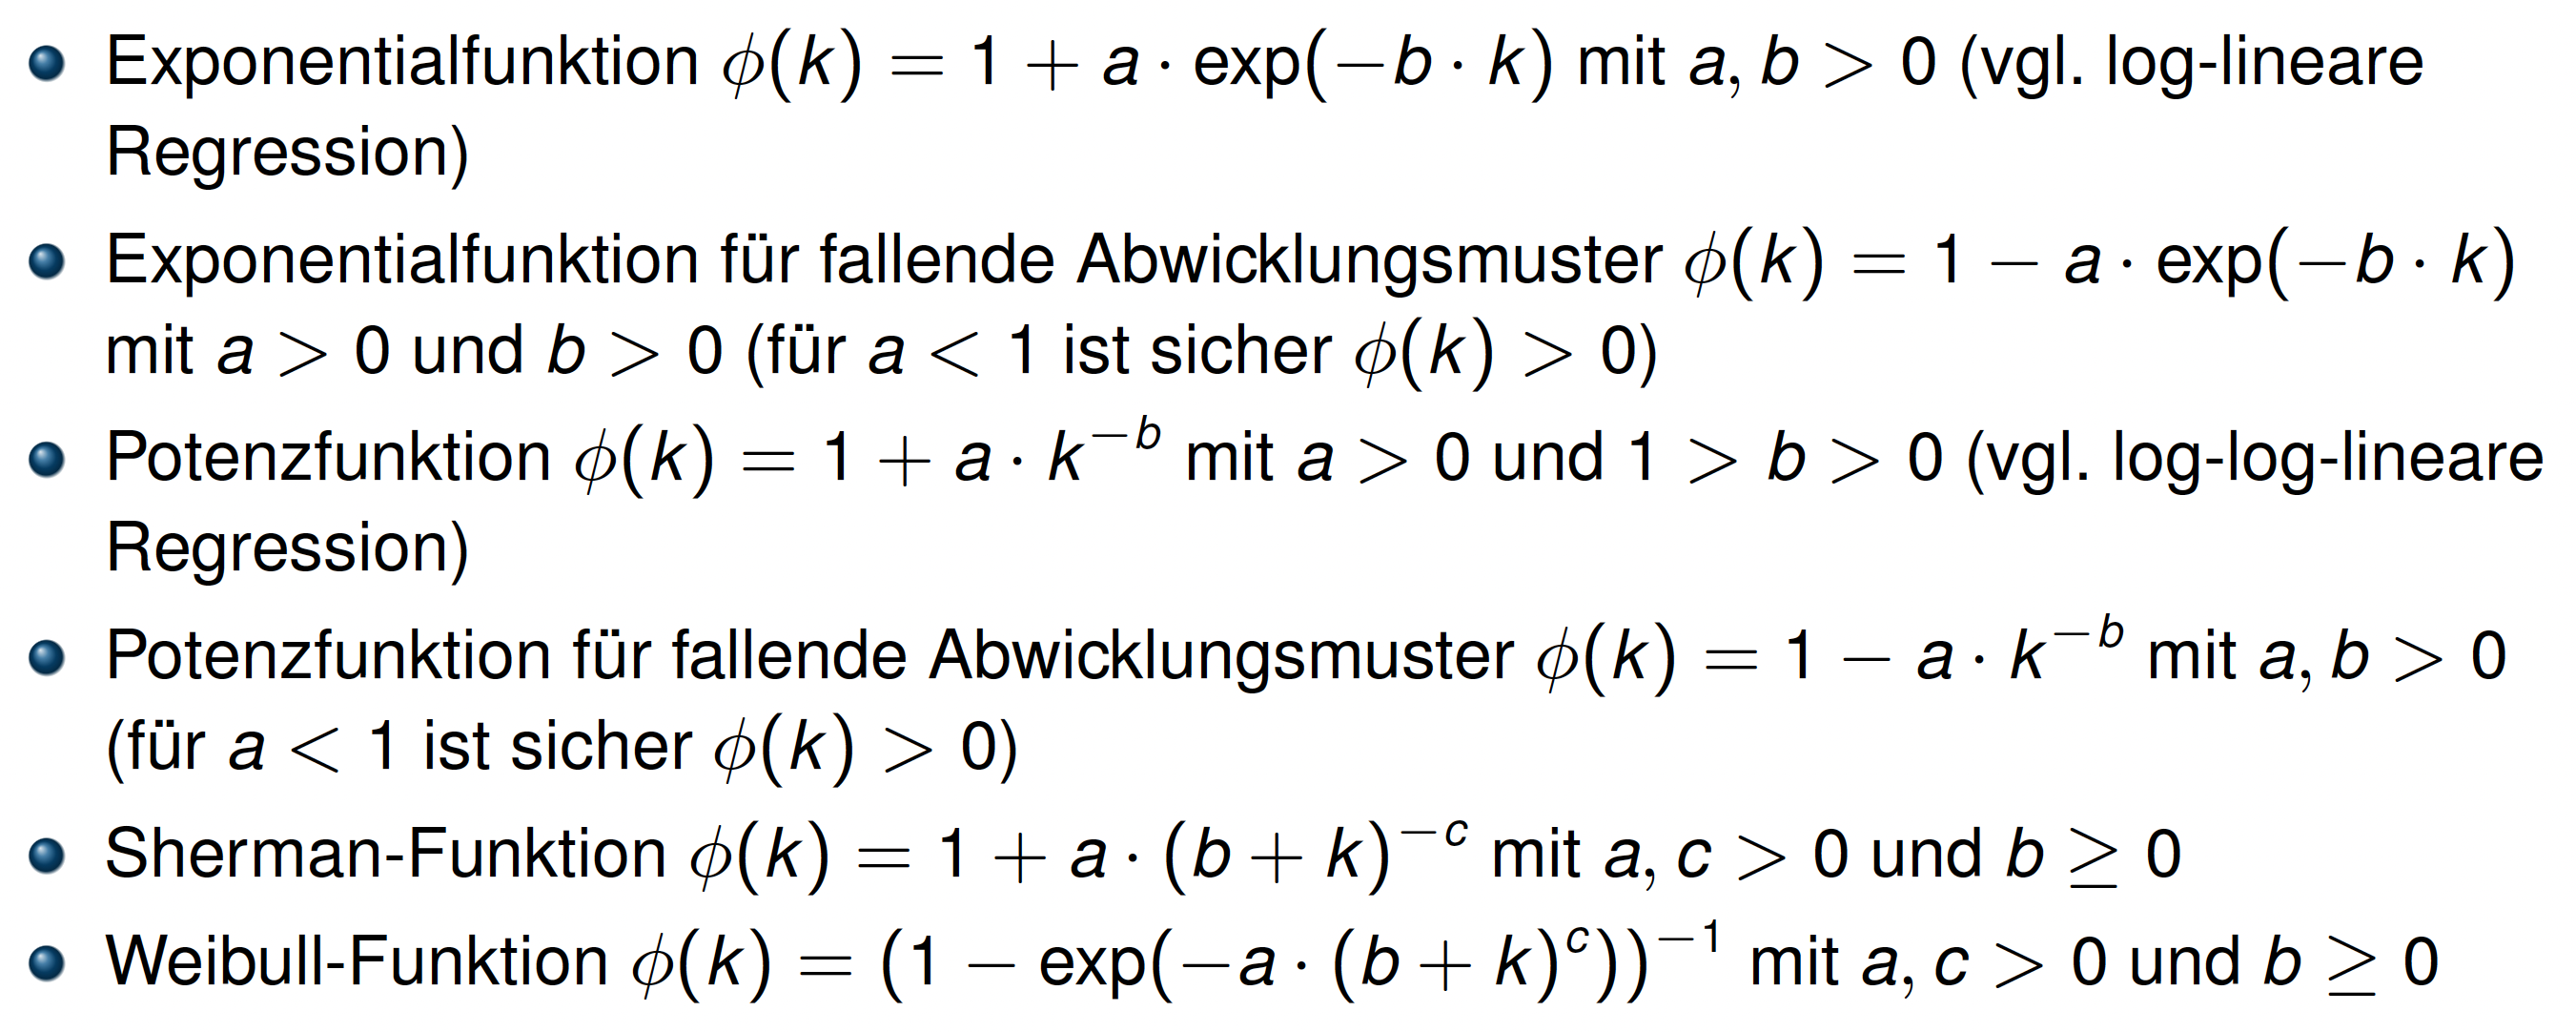
\includegraphics[width=\textwidth]{Bilder/Tailfunktion.png}
\end{figure}

\subsubsection{Sch\"atzung der Tailfaktoren}
\begin{itemize}
	\item [1.] Auswahl einer parametrischen Klasse von Abwicklungsfunktionen $\phi:\mathbb{N} \rightarrow \mathbb{R}_+$
	\item [2.] Auswahl der Abwicklungsjahre $ K \subset \{1,...,n\}$, die verwendet werden sollen
	\item [3.] Sch\"atzung der Parameter von $\phi$ durch Minimieren des gewichteten quadratischen Approximationsfehlers $\sum_{k \in K} w_k (\phi(k) - \hat{f_k})^2$
	\item [4.] $\hat{f_k} := \hat{\phi}(k)$
\end{itemize}

\section{Grundlagen stochastischer Modelle}

\subsection{Sch\"atz-, Zufalls-, und Prognosefehler}
\begin{itemize}
	\item \"Uberpr\"ufung, ob Modellannahmen zu Daten passen
	\item Identifikation nicht angebrachter Methoden
	\item Sinnvoll begr\"undbare Kombination verschiedener Datentypen (z.B. Zahlungen und Aufw\"ande
	\item Berechnung von Zufalls-, Sch\"atz- und Prognosefehlern zur Einsch\"atzung der Unsicherheit
	\item Aggregation der Prognosen und Prognosefehler �ber mehrere Segmente unter Ber\"ucksichtigung von Korrelationen
	\item Simulation der Wahrscheinlichkeitsverteilung
	\item Unvermeidbare Fehler: Modellfehler/\"Anderungsrisiko (au{\ss}erhalb des Modells, Sch\"atzfehler und Zufallsfehler (zusammen Prognosefehler)
	\item \item Wegen der Unsicherheiten in Reserveberichten immer ein Disclaimer
\end{itemize}

\textbf{--------------------------------------
Folie 97 - 129 einbauen?
--------------------------------------}

\subsection{\"Uberpr\"ufung der Modellannahmen und Modellauswahl}

\subsubsection{Graphische Darstellung}

\begin{figure}[H]
\centering
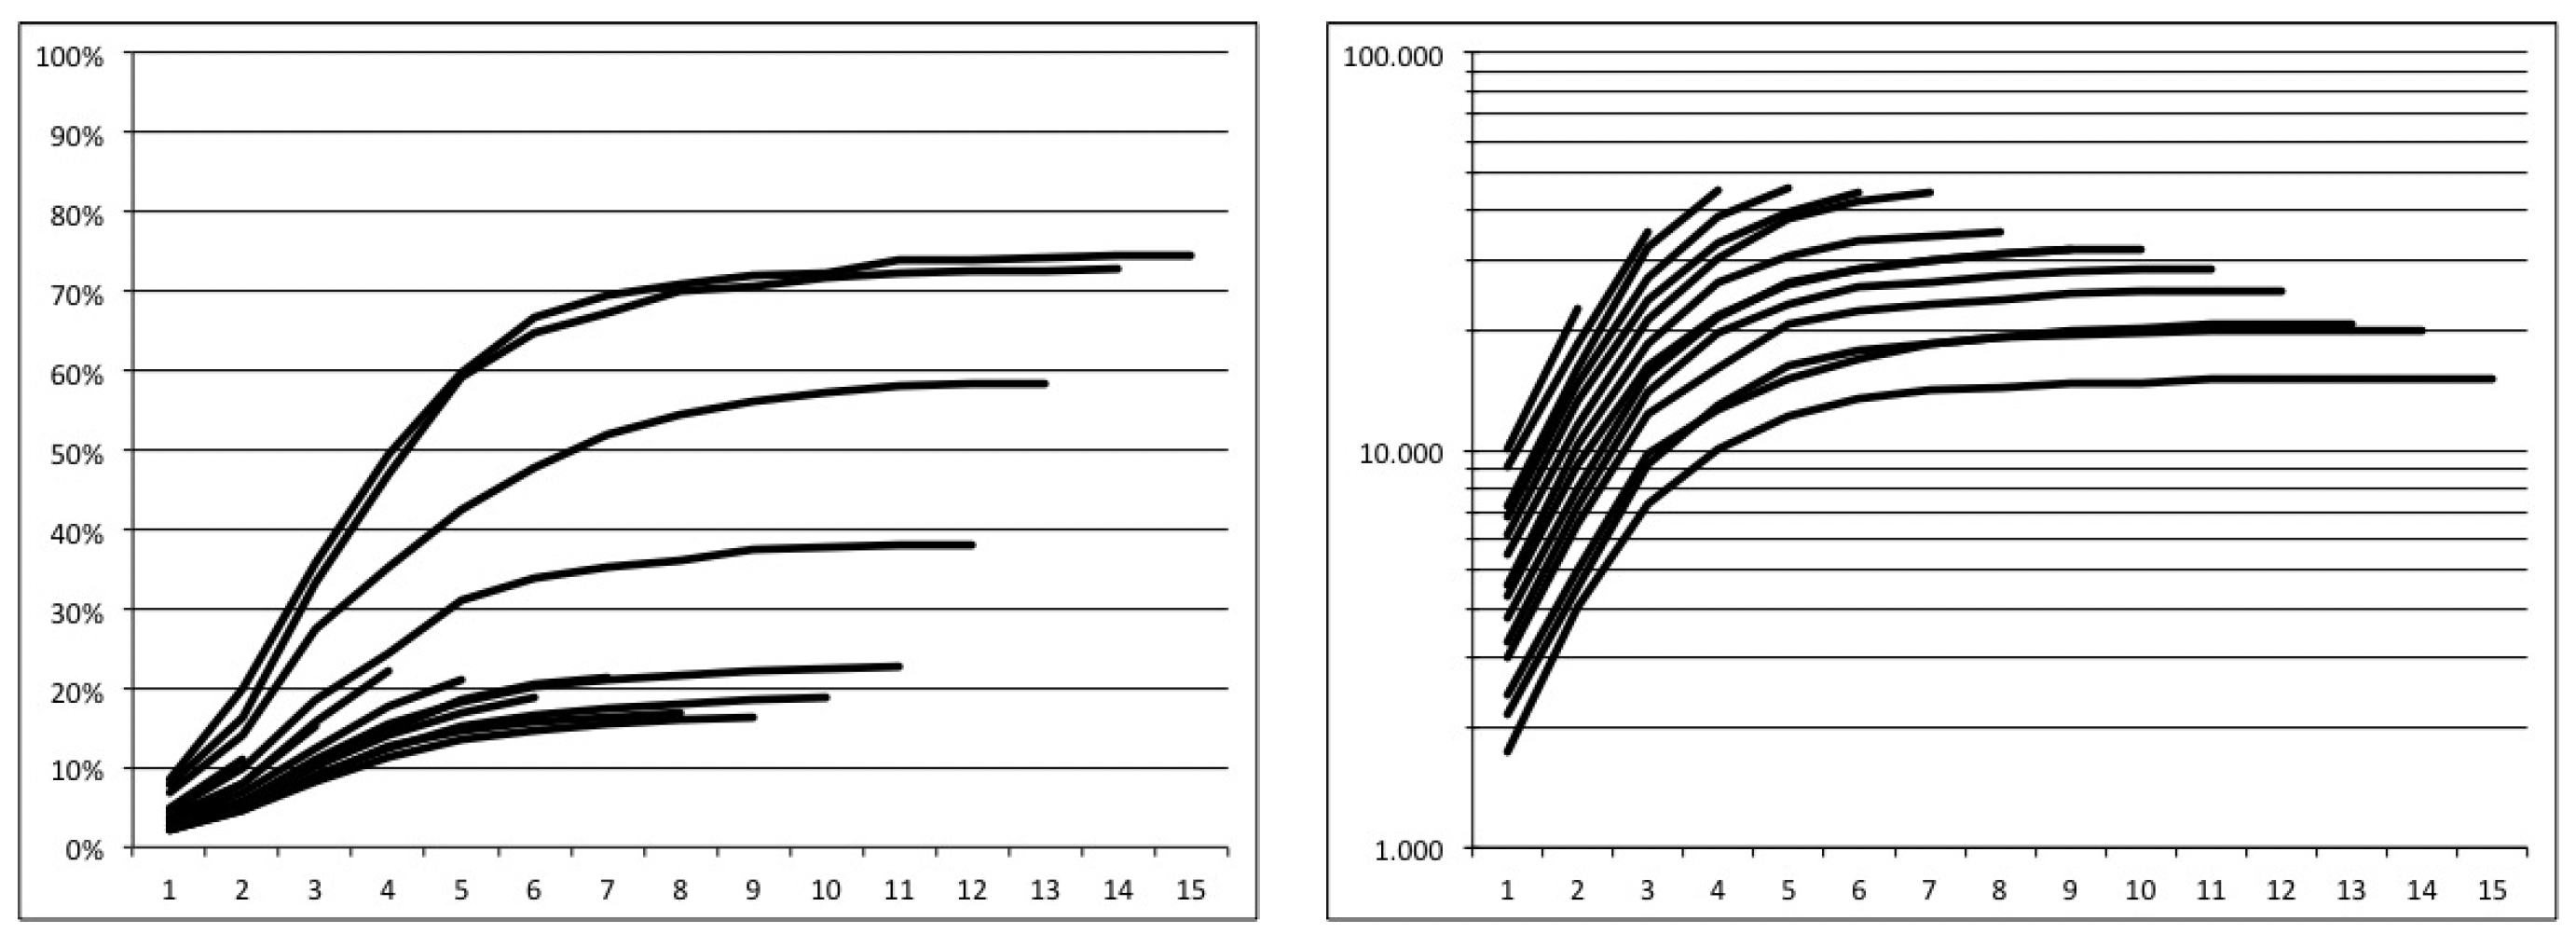
\includegraphics[width=\textwidth]{Bilder/GrafischeDarstellung.png}
\caption{Abwicklung der Anfalljahre, links als Schadenquoten, rechts logarithmusch skalierte Schadenbetr\"age}
\end{figure}

\textbf{Hier gut zu erkennen:}
\begin{itemize}
	\item L\"ange und Form der Abwicklung
	\item Notwendigkeit eines Tails
	\item Volumen\"anderung
	\item Ratenniveau und -\"anderungen
	\item \"Anderung der Portfoliozusammensetzung
	\item Annahme (CL2): Tr\"agt man $C_{i,k}$ f\"ur $i = 1,...,n-k+1$ gegen $C_{i,k-1}$ auf, so sollten die Punkte zu\"allig um die Ursprungsgerade mit Steigung $f_k$ streuen
	\item Stellt man $S_{i,k}$ gegen $C_{i,k-1}$ dar, so gilt die Aussage analog mit Steigung $f_k - 1$
	\item Bei ILR2: in der grafischen Darstellung von $S_{i,k}$ gegen $v_i$ f\"ur $i=1,...,n-k+1$ streuen die Punkte zu\"allig um die Ursprungsgerade mit Steigung $m_k$ (siehe Grafik)
\end{itemize}

\begin{figure}[H]
\centering
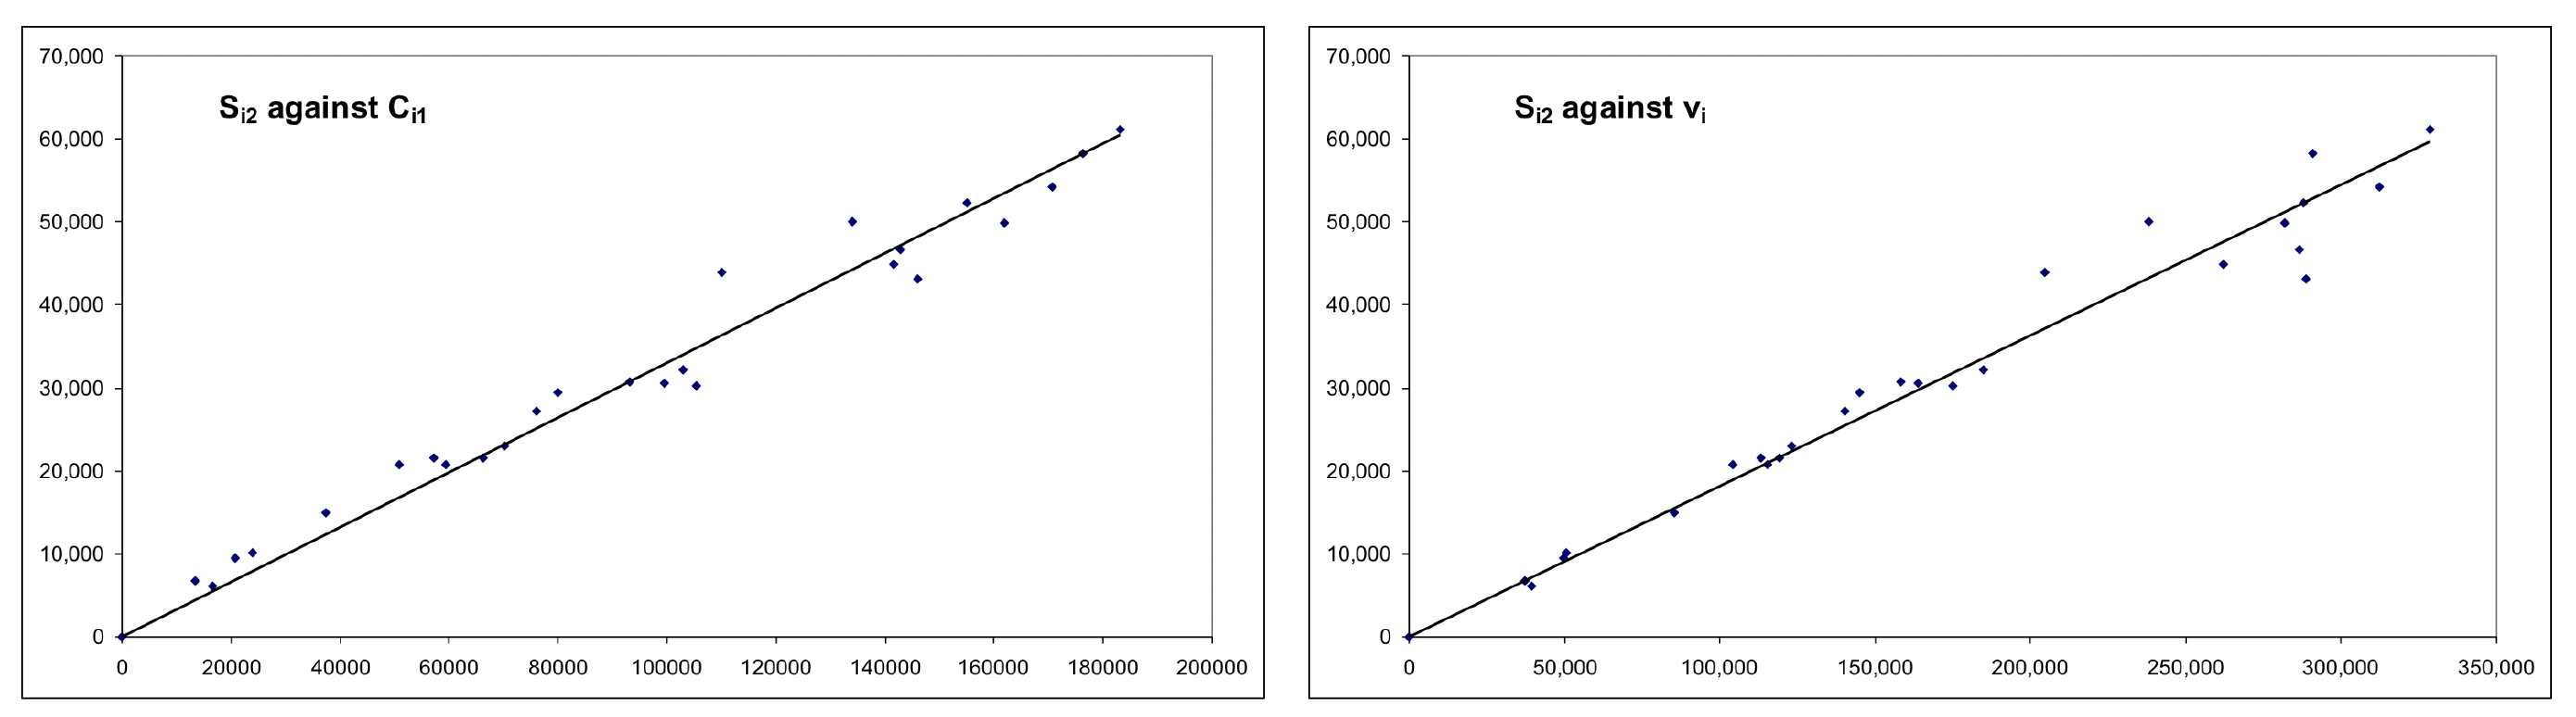
\includegraphics[width=\textwidth]{Bilder/Streuung.png}
\end{figure}

\subsubsection{Residuenanalyse}

\begin{itemize}
	\item Residuen beschreiben Abweichungen vom Mittelwert in normierter Art
	\item Idealfall: wei{\ss}es Rauschen
	\item Sch\"atzungen: 
\end{itemize}

\begin{figure}[H]
\centering
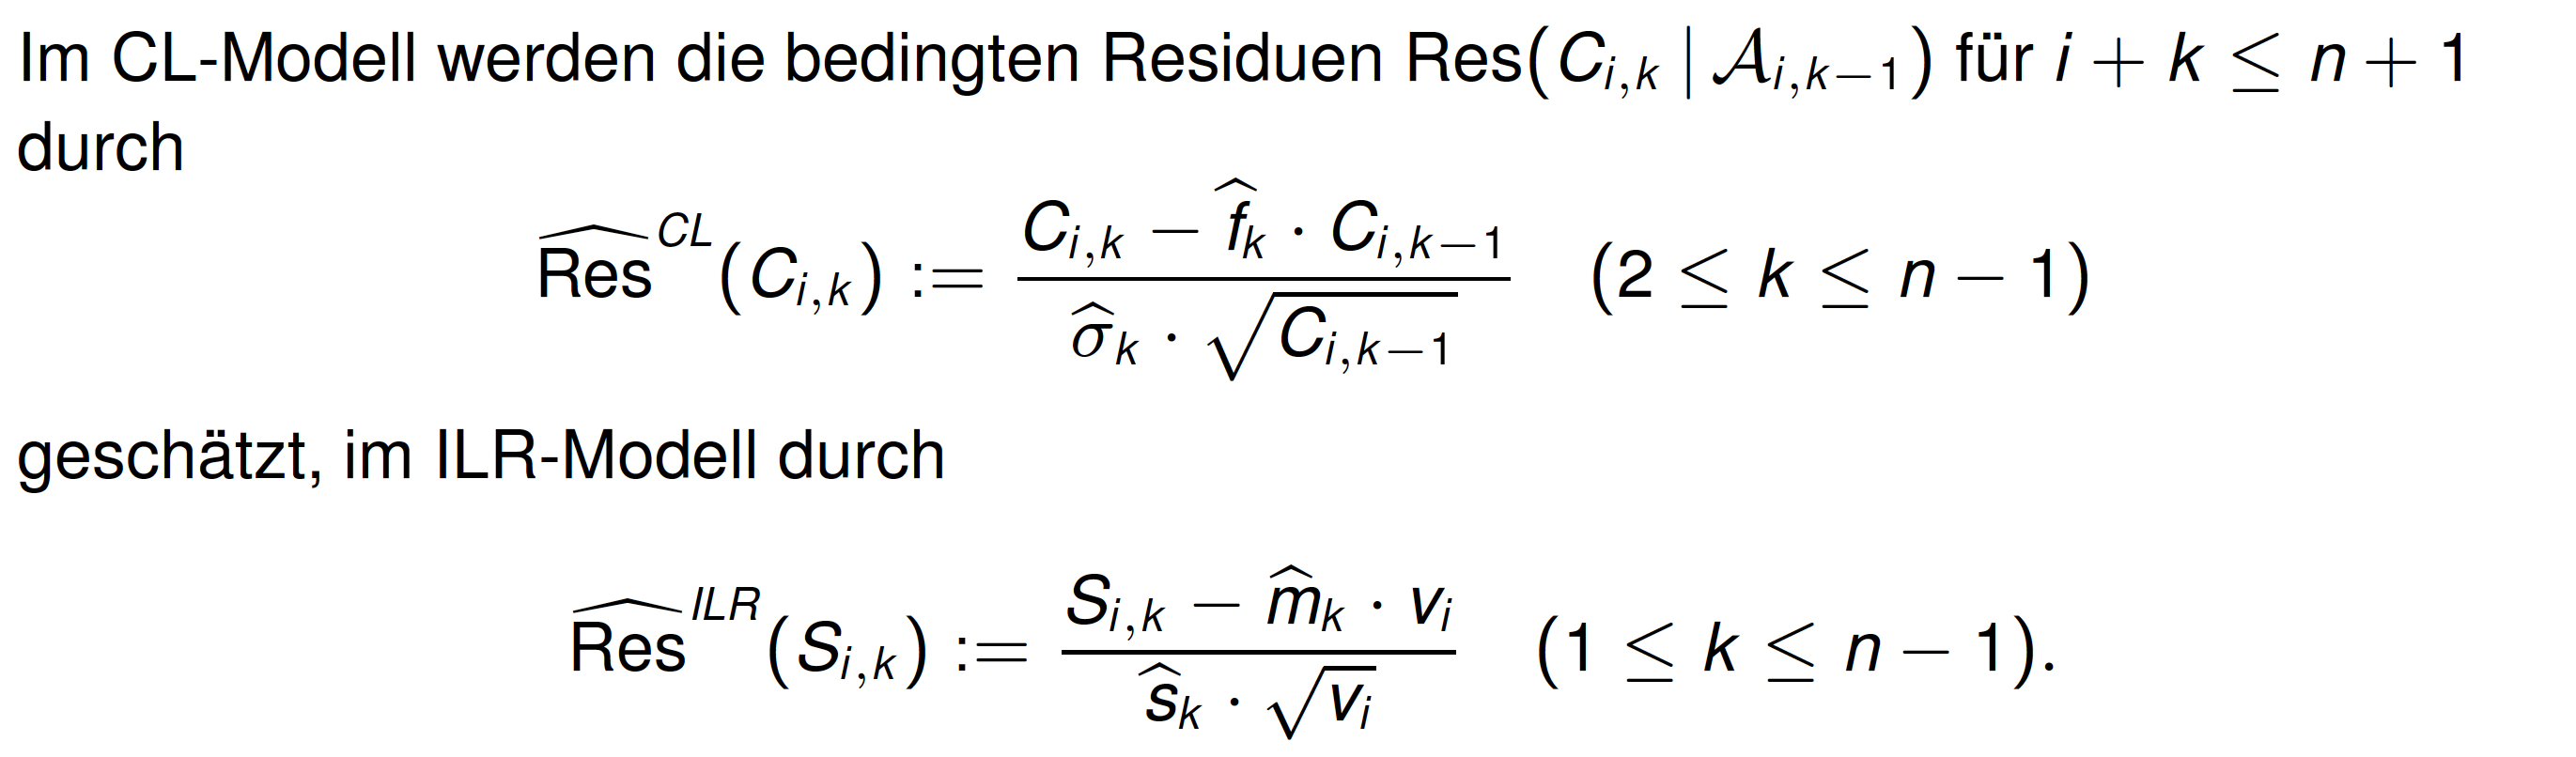
\includegraphics[width=\textwidth]{Bilder/Schaetzungen.png}
\end{figure}

\begin{itemize}
	\item Summenformel f\"ur Residuenquadrate: $ \sum_{i=1}^{n-k+1} \widehat{Res}^{CL}(C_{i,k})^2 = n - k = \sum_{i=1}^{n-k+1} \widehat{Res}^{ILR}(S_{i,k})^2$
	\item Auswirkungen der Summenformel f\"ur Residuenquadrate:
	\begin{itemize}
		\item Betrag der gesch\"atzten Residuen durch $\sqrt{n-k}$ begrenzt
		\item Je h\"oher das Jahr, desto kleiner die maximal m\"oglichen Betr\"age
		\item Sch\"atzung der Residuen in der rechten Spitze des Dreiecks beruht nur auf wenigen Daten, daher kaum Aussagekraft
	\end{itemize}
\end{itemize}

\subsubsection{Graphische Residuenanalyse}
\begin{itemize}
	\item unterschiedliche Abwicklungsfaktoren der verschiedenen Abwicklungsjahre durch Residuen vergleichbar
	\item Residuen gegen Abwicklungsjahr: Streuen nach Konstruktion um Null, idealerweise wei{\ss}es Rauschen
	\item Residuen gegen Anfalljahr: \"anderungen des Abwicklungsverhaltens aufgrund Portfoliozusammensetzung oder Raten\"anderung (nur ILR)
	\item Residuen gegen Kalenderjahr: Pl\"otzliche oder graduelle Kalenderjahreseffekte
	\item Beispiele siehe Folien 137 - 140
	\item Wichtig: Residuen des j\"ungsten Kalenderjahres f\"ur aktuelle Trends 
\end{itemize}

\subsubsection{Auswahl eines Modells}
\begin{itemize}
	\item Parallelenkriterium:
	\begin{itemize}
		\item ILR-Fall f\"ur ein festes Abwicklungsjahr k: $\frac{C_{i,k}}{v_i} - \frac{C_{i,k-1}}{v_i} = \frac{S_{i,k}}{v_i} \thickapprox m_k$, d.h. Stegungen der AJ ann\"ahern parallel
		\item CL-Fall f\ur festes Abwicklungsjahr k: $ln(\frac{C_{i,k}}{v_i}) - ln(\frac{C_{i,k-1}}{v_i}) = ln(\frac{C_{i,k}}{C_i,k-1}}) \thickapprox ln(f_k)$, d.h. Steigung der AJ mit logarithmisch skalierter y-Achse ann\"ahernd parallel.
	\end{itemize}
	\item Backtesting-Kriterium
	\begin{itemize}
		\item \"Uberpr\"ufung, welches Modell in der beobachteten Vergangenheit eines Abwicklungsjahres $k$ mit $2 \leq k \leq n-1$ die genaueren Prognosen geliefert h\"atte
		\item Berechne daf\"ur Differenzen $S_{i,k} - (\hat{f}_k - 1) \cdot C_{i,k-1}$ und $S_{i,k} - \hat{m}_k \cdot v_i$
		\item Sieger: kleinerer Differenzbetrag
		\item Dreieck entsprechend einf\"arben $\rightarrow$ gemustertes Bild
		\item Kombination:  f\"ur verschiedene Abwicklungsjahre unterschiedliche Modelle w\"ahlen, nicht zu h\"aufig wechseln
	\end{itemize}
	\item Korrelationskriterium
	\begin{itemize}
		\item IRL: $Cov(\frac{C_{i,k-1}}{v_i},\frac{S_{i,k}}{v_i})=0$ und $Cov^{\mathcal{A}_{i,k-1}}(\frac{C_{i,k}}{C_{i,k-1}},\frac{C_{i,k+1}}{C_{i,k}}) <0$
		\item CL: $Cov(\frac{C_{i,k-1}}{v_i},\frac{S_{i,k}}{v_i})=Var(C_{i,k-1}) \cdot \frac{f_k-1}{v_i^2}$ und $Cov^{\mathcal{A}_{i,k-1}}(\frac{C_{i,k}}{C_{i,k-1}},\frac{C_{i,k+1}}{C_{i,k}}) = 0$
		\item Zugangsquoten und Schadenquoten unkorreliert (positiv korreliert) und sukzessive Abwicklungsfaktoren negativ korreliert (unkorreliert), so spricht dies f\"ur das ILR-Modell (CL-Modell)
	\end{itemize}
\end{itemize}

\subsection{Aggregation der Reserven mehrerer Segmente}

\begin{itemize}
	\item Portfolio \"ublicherweise bestehend aus mehreren Segmenten
	\item $D_{i,k}$ f\"ur $i=1,...,n$ und $k=1,...,u$ die kumulierten Schadenst\"ande eines weiteren Segments
	\item $R_i^C$, $R_j^D$ die jeweiligen Reserven, $v_i^C$, $v_i^D$ die Volumina
	\item Annahme: zwei Segmente der gleichen Gr"o{\ss}e
\end{itemize}


\subsubsection{Gesamtreserve}
\begin{itemize}
	\item nicht additiv: $\hat{R}_i^{C+D} \neq \hat{R}_i^C + \hat{R}_i^D$
	\item in der Praxis gilt das irgendwie doch??? Keine Ahnung, Folie 151
	\item Zur bestimmung der (bedingten) Varianzen von $R_i^C+R_i^D$ bzw. $\hat{R}_i^C + \hat{R}_i^D$ braucht man die Kovarianzen zwischen diesen Gr\"o{\ss}en
	\item Analyse der Korrelationen mit Residuen
\end{itemize}


\subsubsection{Korrelationsmodell zur Aggregation von Reserven nach Braun 2004}

\begin{figure}[H]
\centering
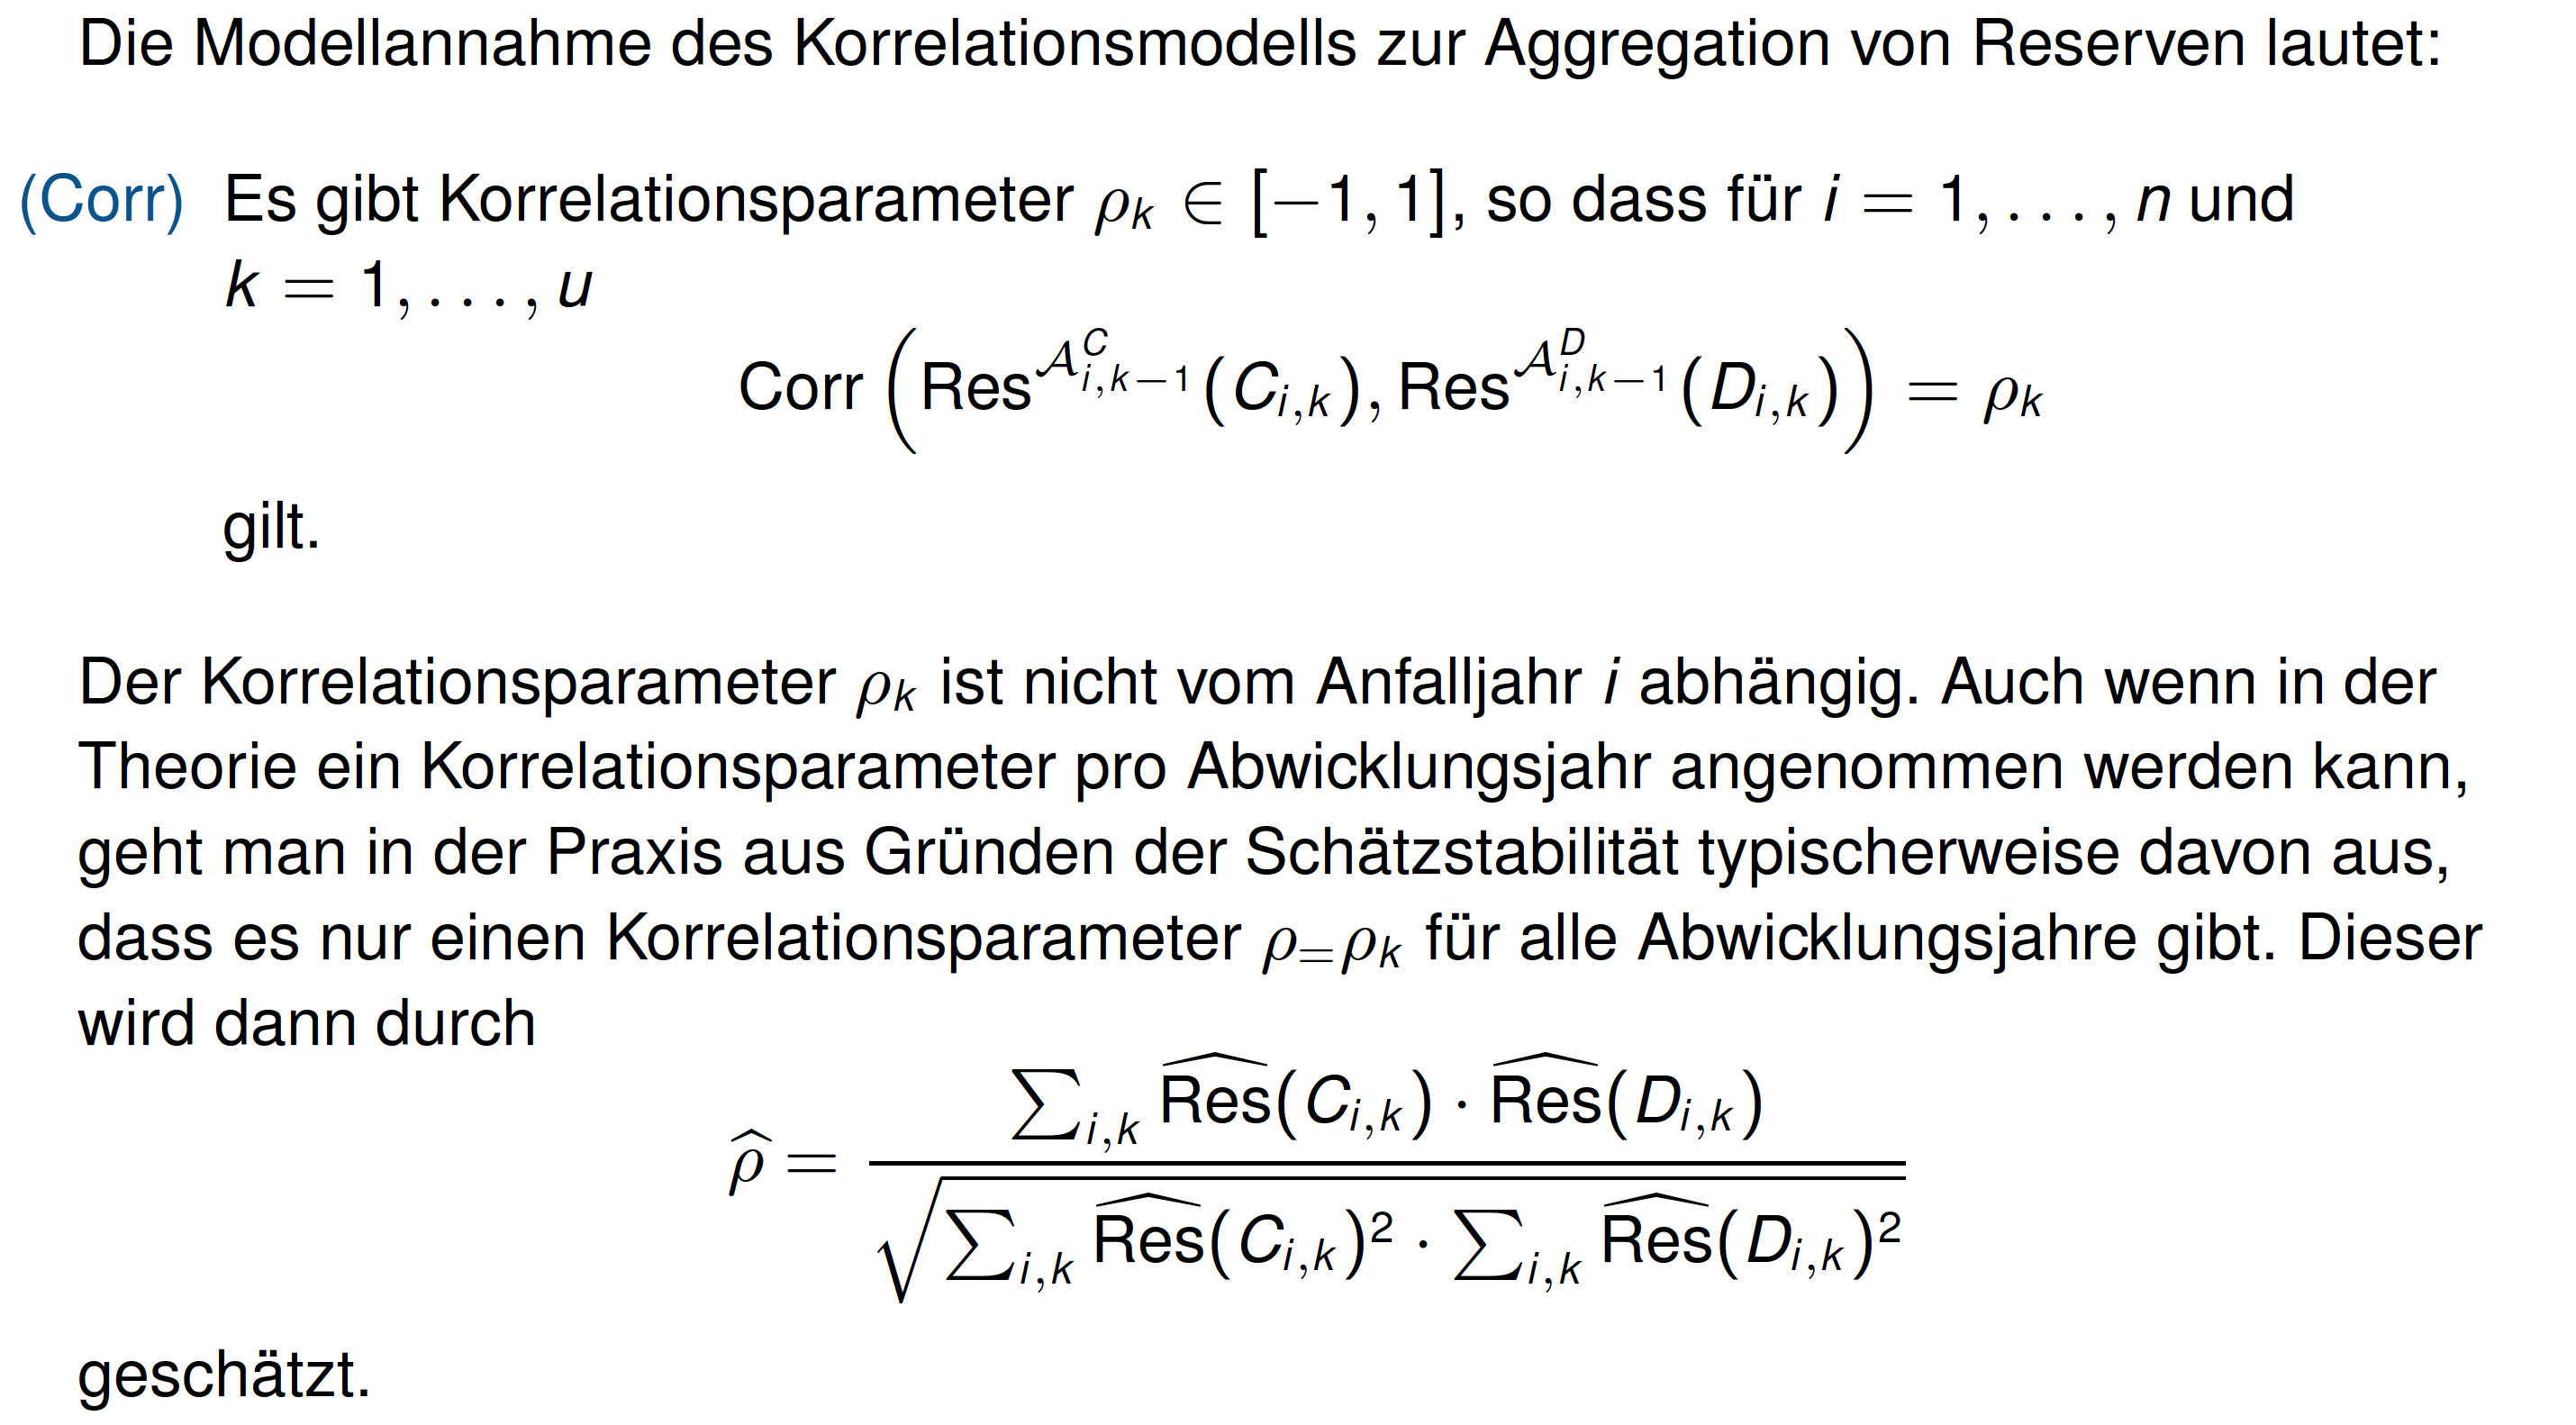
\includegraphics[width=\textwidth]{Bilder/Braun1.png}
\end{figure}

\textbf{Bemerkungen:}
\begin{itemize}
	\item Abh\"angigkeit der Residuensch\"atzer ist eine Unsicherheitsquelle bei der Bestimmung des Korrelationsparameters
	\item Durch Summenformel f\"ur Residuenquadrate: unsichere Residuen haben keinen gro{\ss}en Einfluss
\end{itemize}

\begin{figure}[H]
\centering
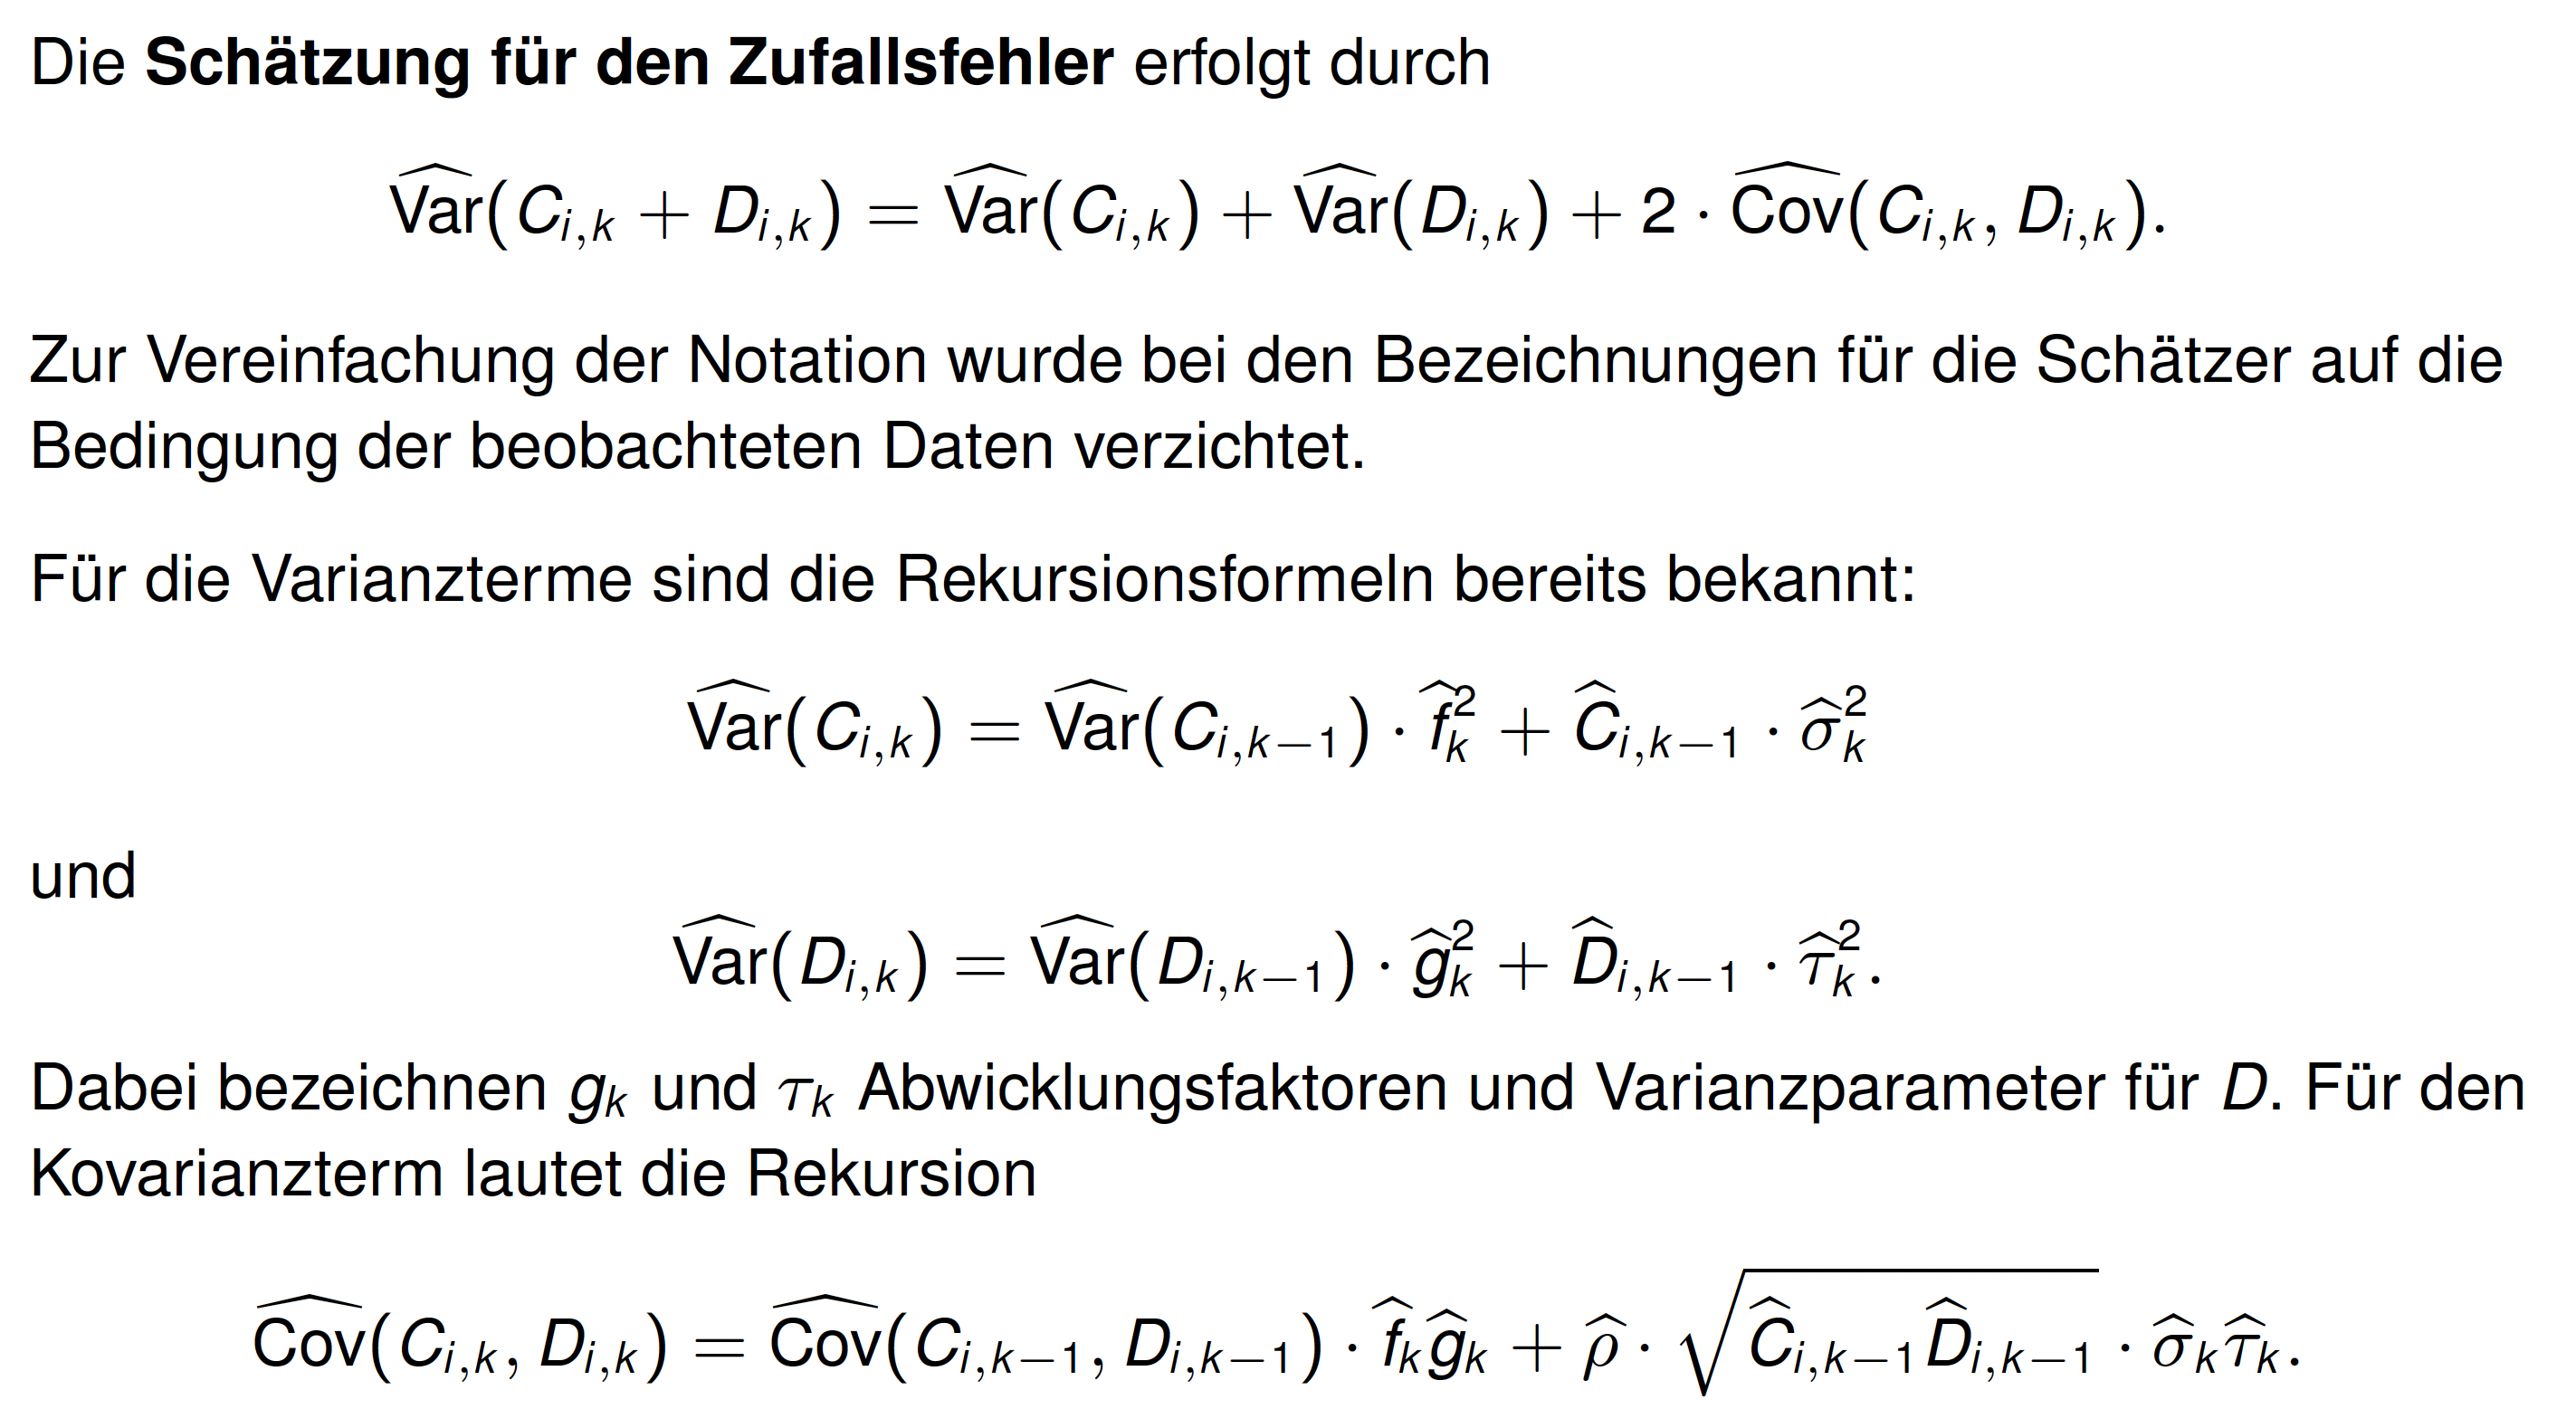
\includegraphics[width=\textwidth]{Bilder/Braun2.png}
\end{figure}

\begin{figure}[H]
\centering
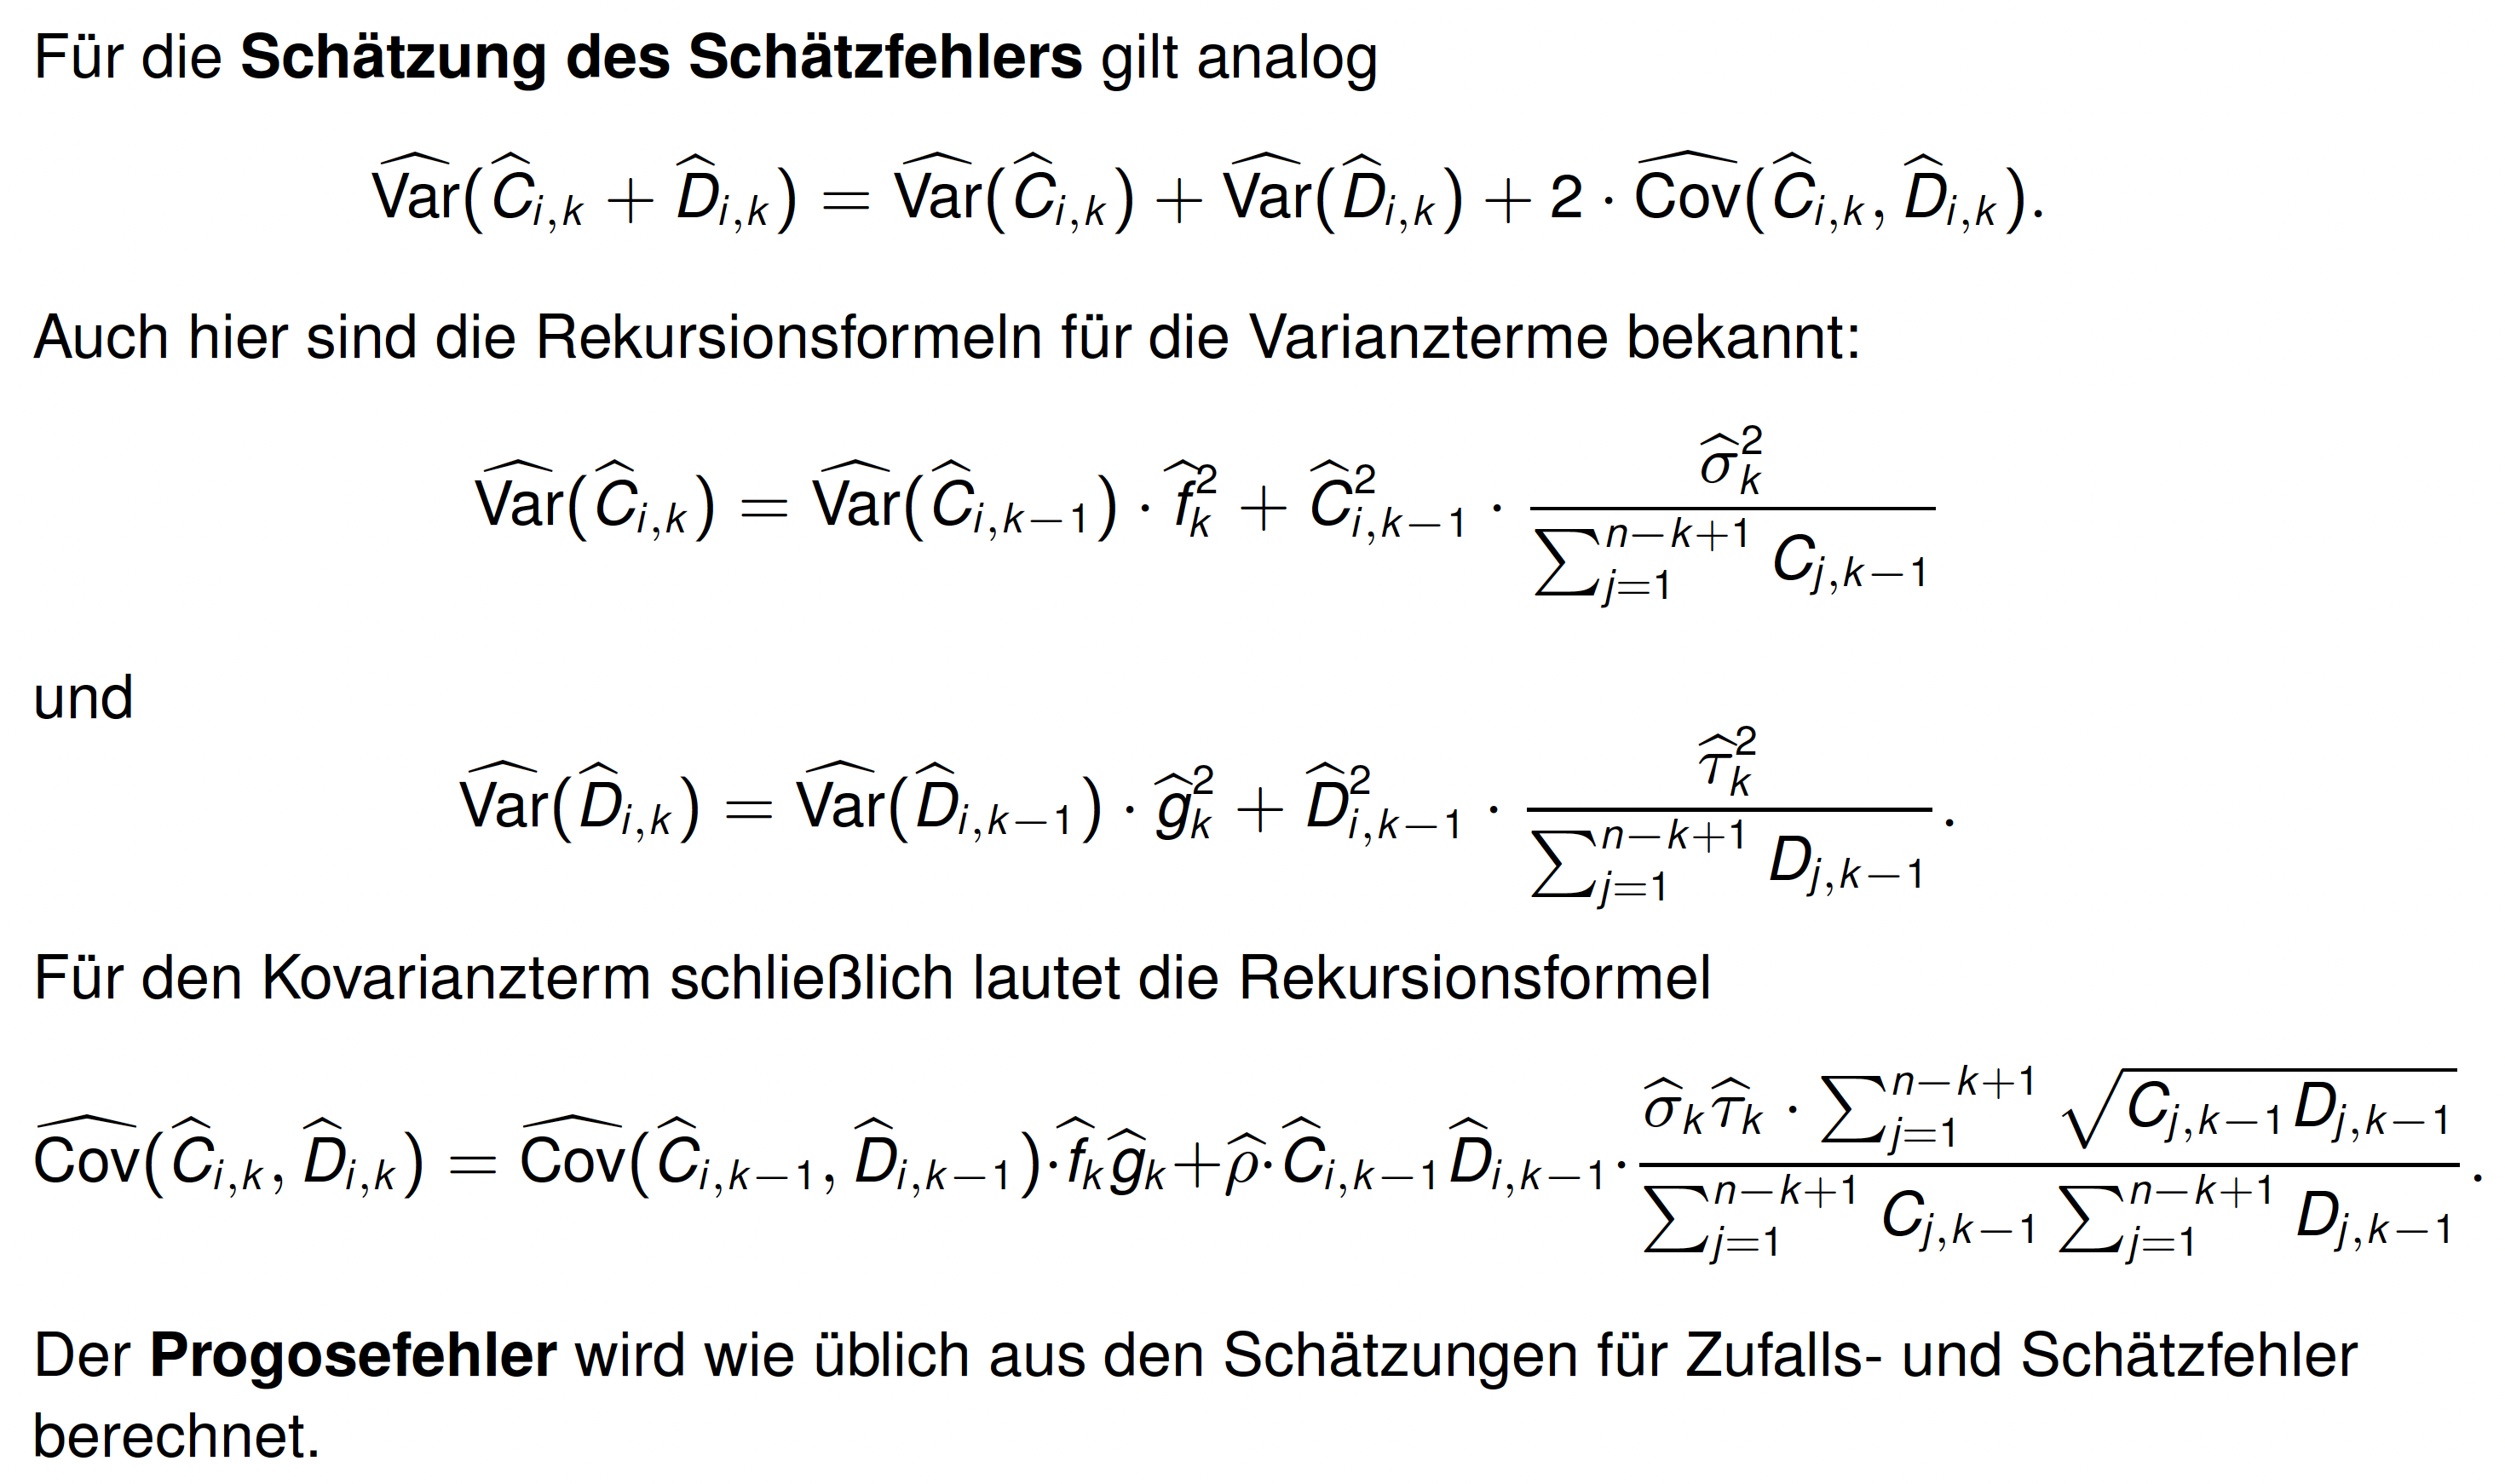
\includegraphics[width=\textwidth]{Bilder/Braun3.png}
\end{figure}

\subsubsection{Bemerkungen zum Korrelationsmodell}

\textbf{Sch\"atzungen der Korrelationsparameter}
\begin{itemize}
	\item Sch\"atzungen der Korrelationsparameter
	\begin{itemize}
		\item Sch\"atzung eines Korrelationsparameters pro Abwicklungsjahr nicht sinnvoll
		\item Stabilisierung durch Analyse auf der Ebene von Ausweisbranchen
	\end{itemize}
	\item Folgerungen f\"ur Korrelationsstruktur
	\begin{itemize}
		\item es gibt keinen Korrelationskoeffizienten zwischen den Reserven zweier Segmente, der durch die Segmente alleine bestimmt ist
		\item Korrelation zwischen Reserven und Reservesch\"atzern h\"angt z.B. von der Verteilung der AJ ab
		\item Verwendung eines externen Koeffizienten ist einfacher
	\end{itemize}
\end{itemize}


\subsection{Bornhuetter/Ferguson-Modell}

\subsubsection{Das Verfahren}

\begin{figure}[H]
\centering
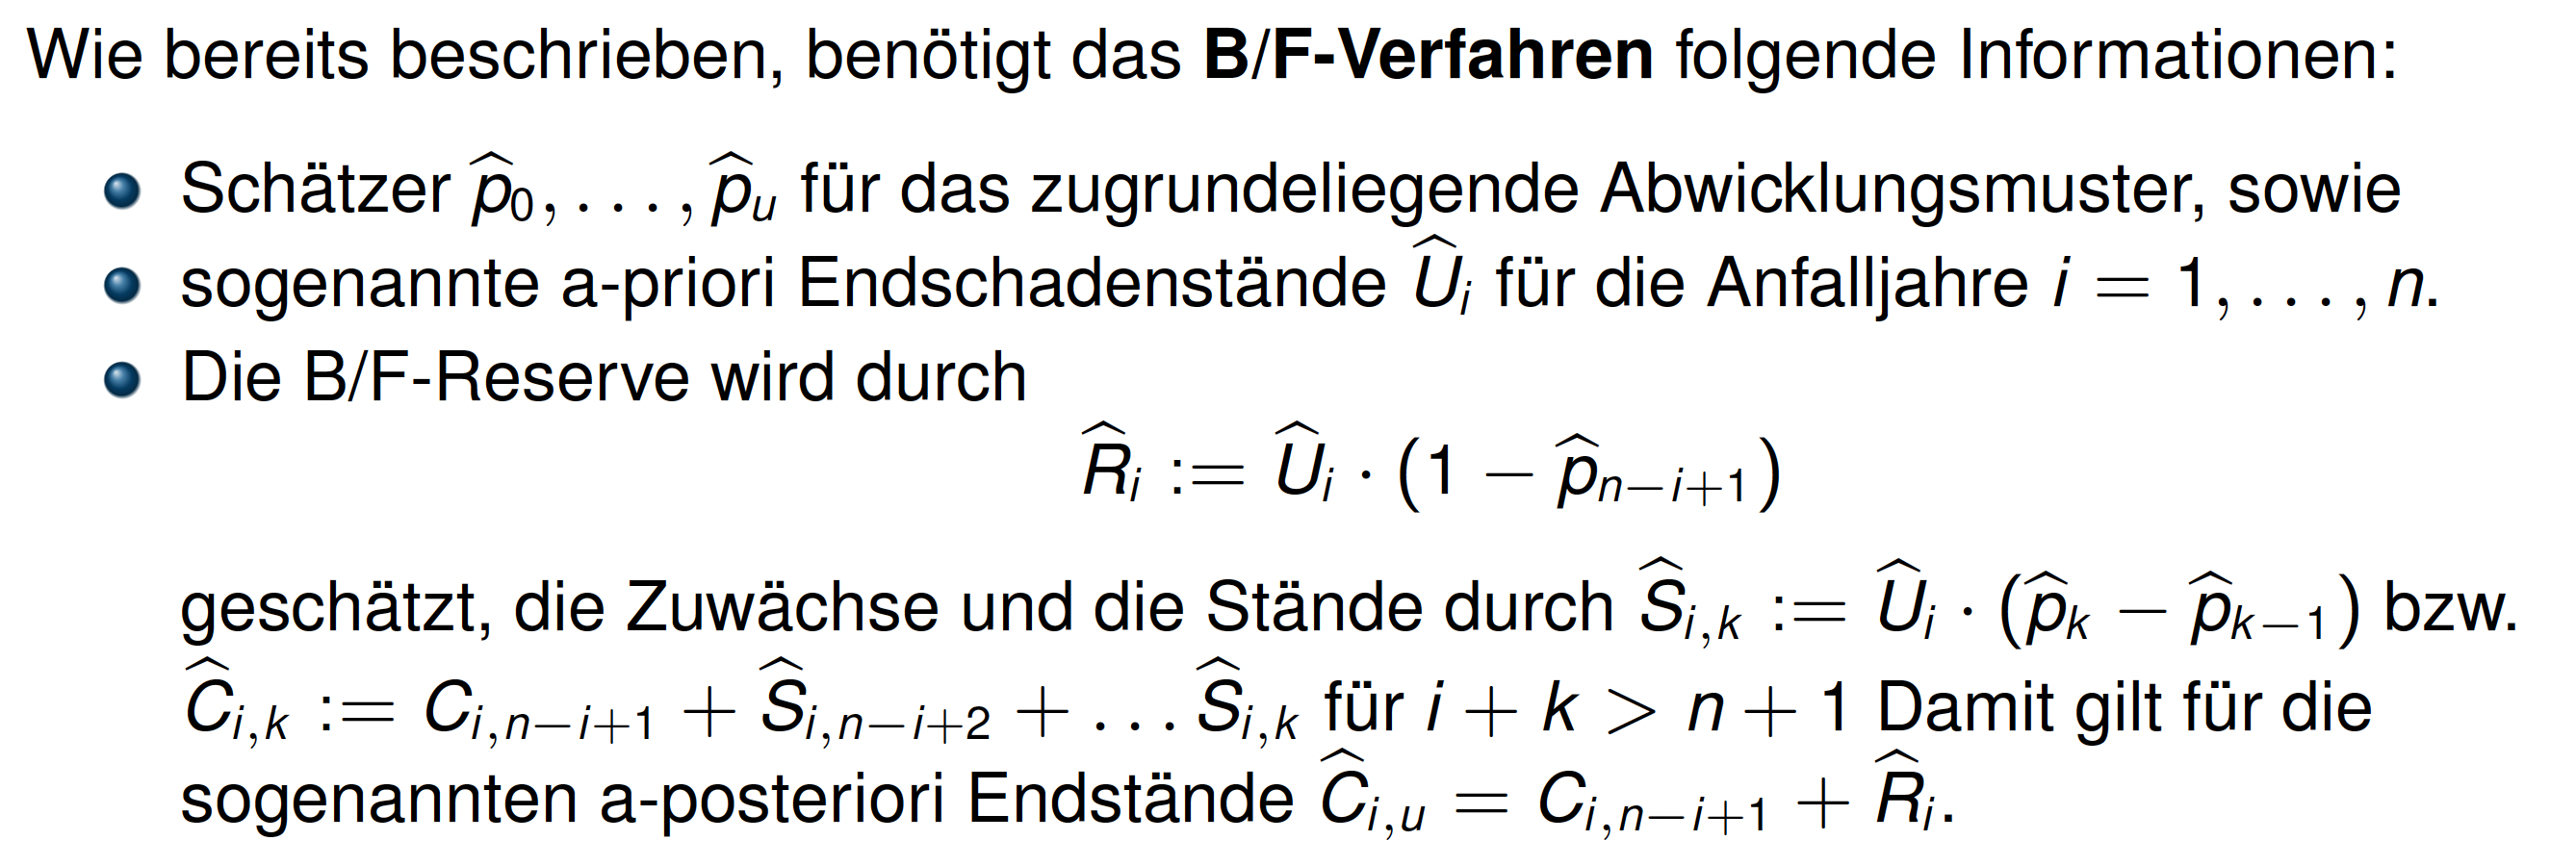
\includegraphics[width=\textwidth]{Bilder/BF.png}
\end{figure}

\subsubsection{Eigenschaften B/F-Methode}
\begin{itemize}
	\item a-priori Endschadenstand $\hat{U}_i$ meist als Endschadenquote $\hat{q}_i$ \"uber $\hat{U}_i = \hat{q}_i \cdot v_i$ f\"ur $i = 1,...,n$ gegeben
	\item initiale Schadenquote $\hat{q}_i$ f\"ur j\"ungere Anfalljahre meist aus Tarifierung und Pricing
	\item F\"ur \"altere Jahre oft nicht vorhanden oder aus Vorjahr \"ubernommen
	\item $\hat{C}_{i,u} - \hat{U}_i = C_{i,n-i+1} + \hat{R}_i - \hat{U}_i \cdot (\hat{p}_{n-i+1} + (1- \hat{p}_{n-i+})) = C_{i,n-i+1} - \hat{U}_i \cdot \hat{p}_{n-i+1}$ verschwindet genau dann, wenn aktueller Stand zur Erwartung passt
\end{itemize}

\begin{figure}[H]
\centering
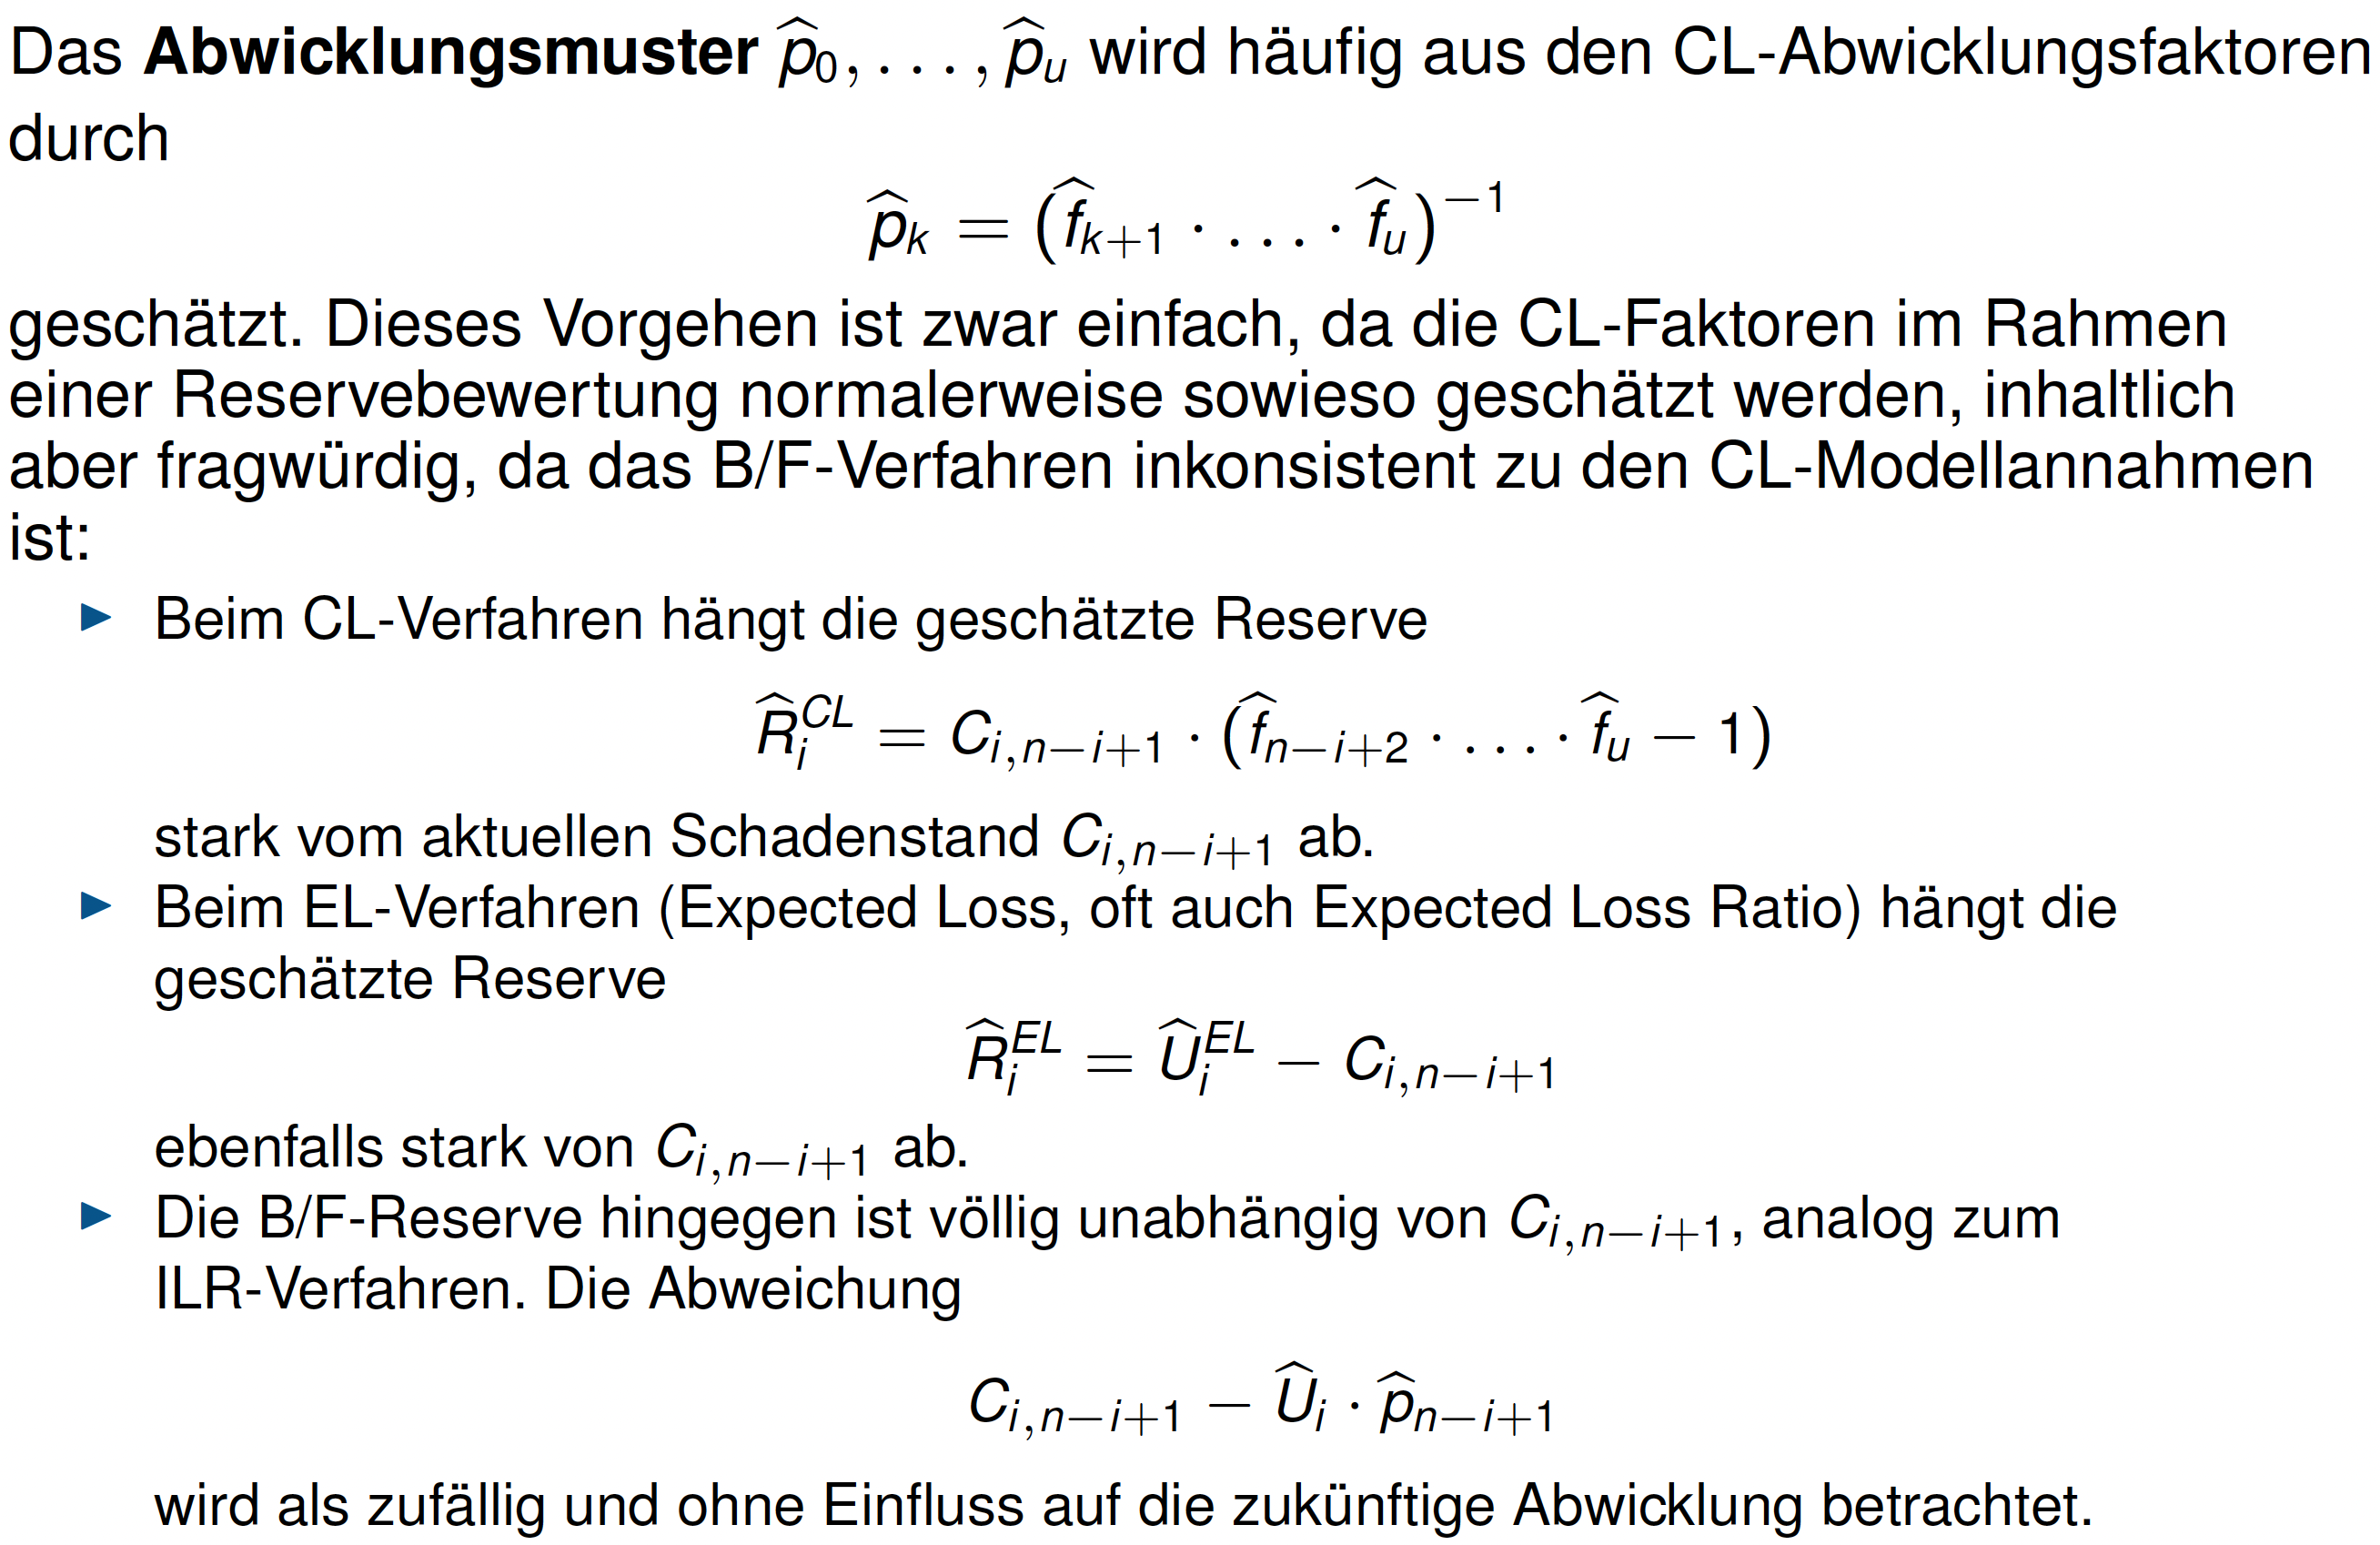
\includegraphics[width=\textwidth]{Bilder/BF2.png}
\end{figure}

\begin{itemize}
	\item Unabh\"angigkeit des aktuellen Schadenstandes von der gesch\"atzten B/F-Reserve ist fundamentale Eigenschaft des B/F-Verfahrens
	\item B/F und ILR sehr \"ahnlich, Reserve kann \"ubereinstimmen 
\end{itemize}


\subsubsection{Modell Annahmen nach Mack}

\begin{figure}[H]
\centering
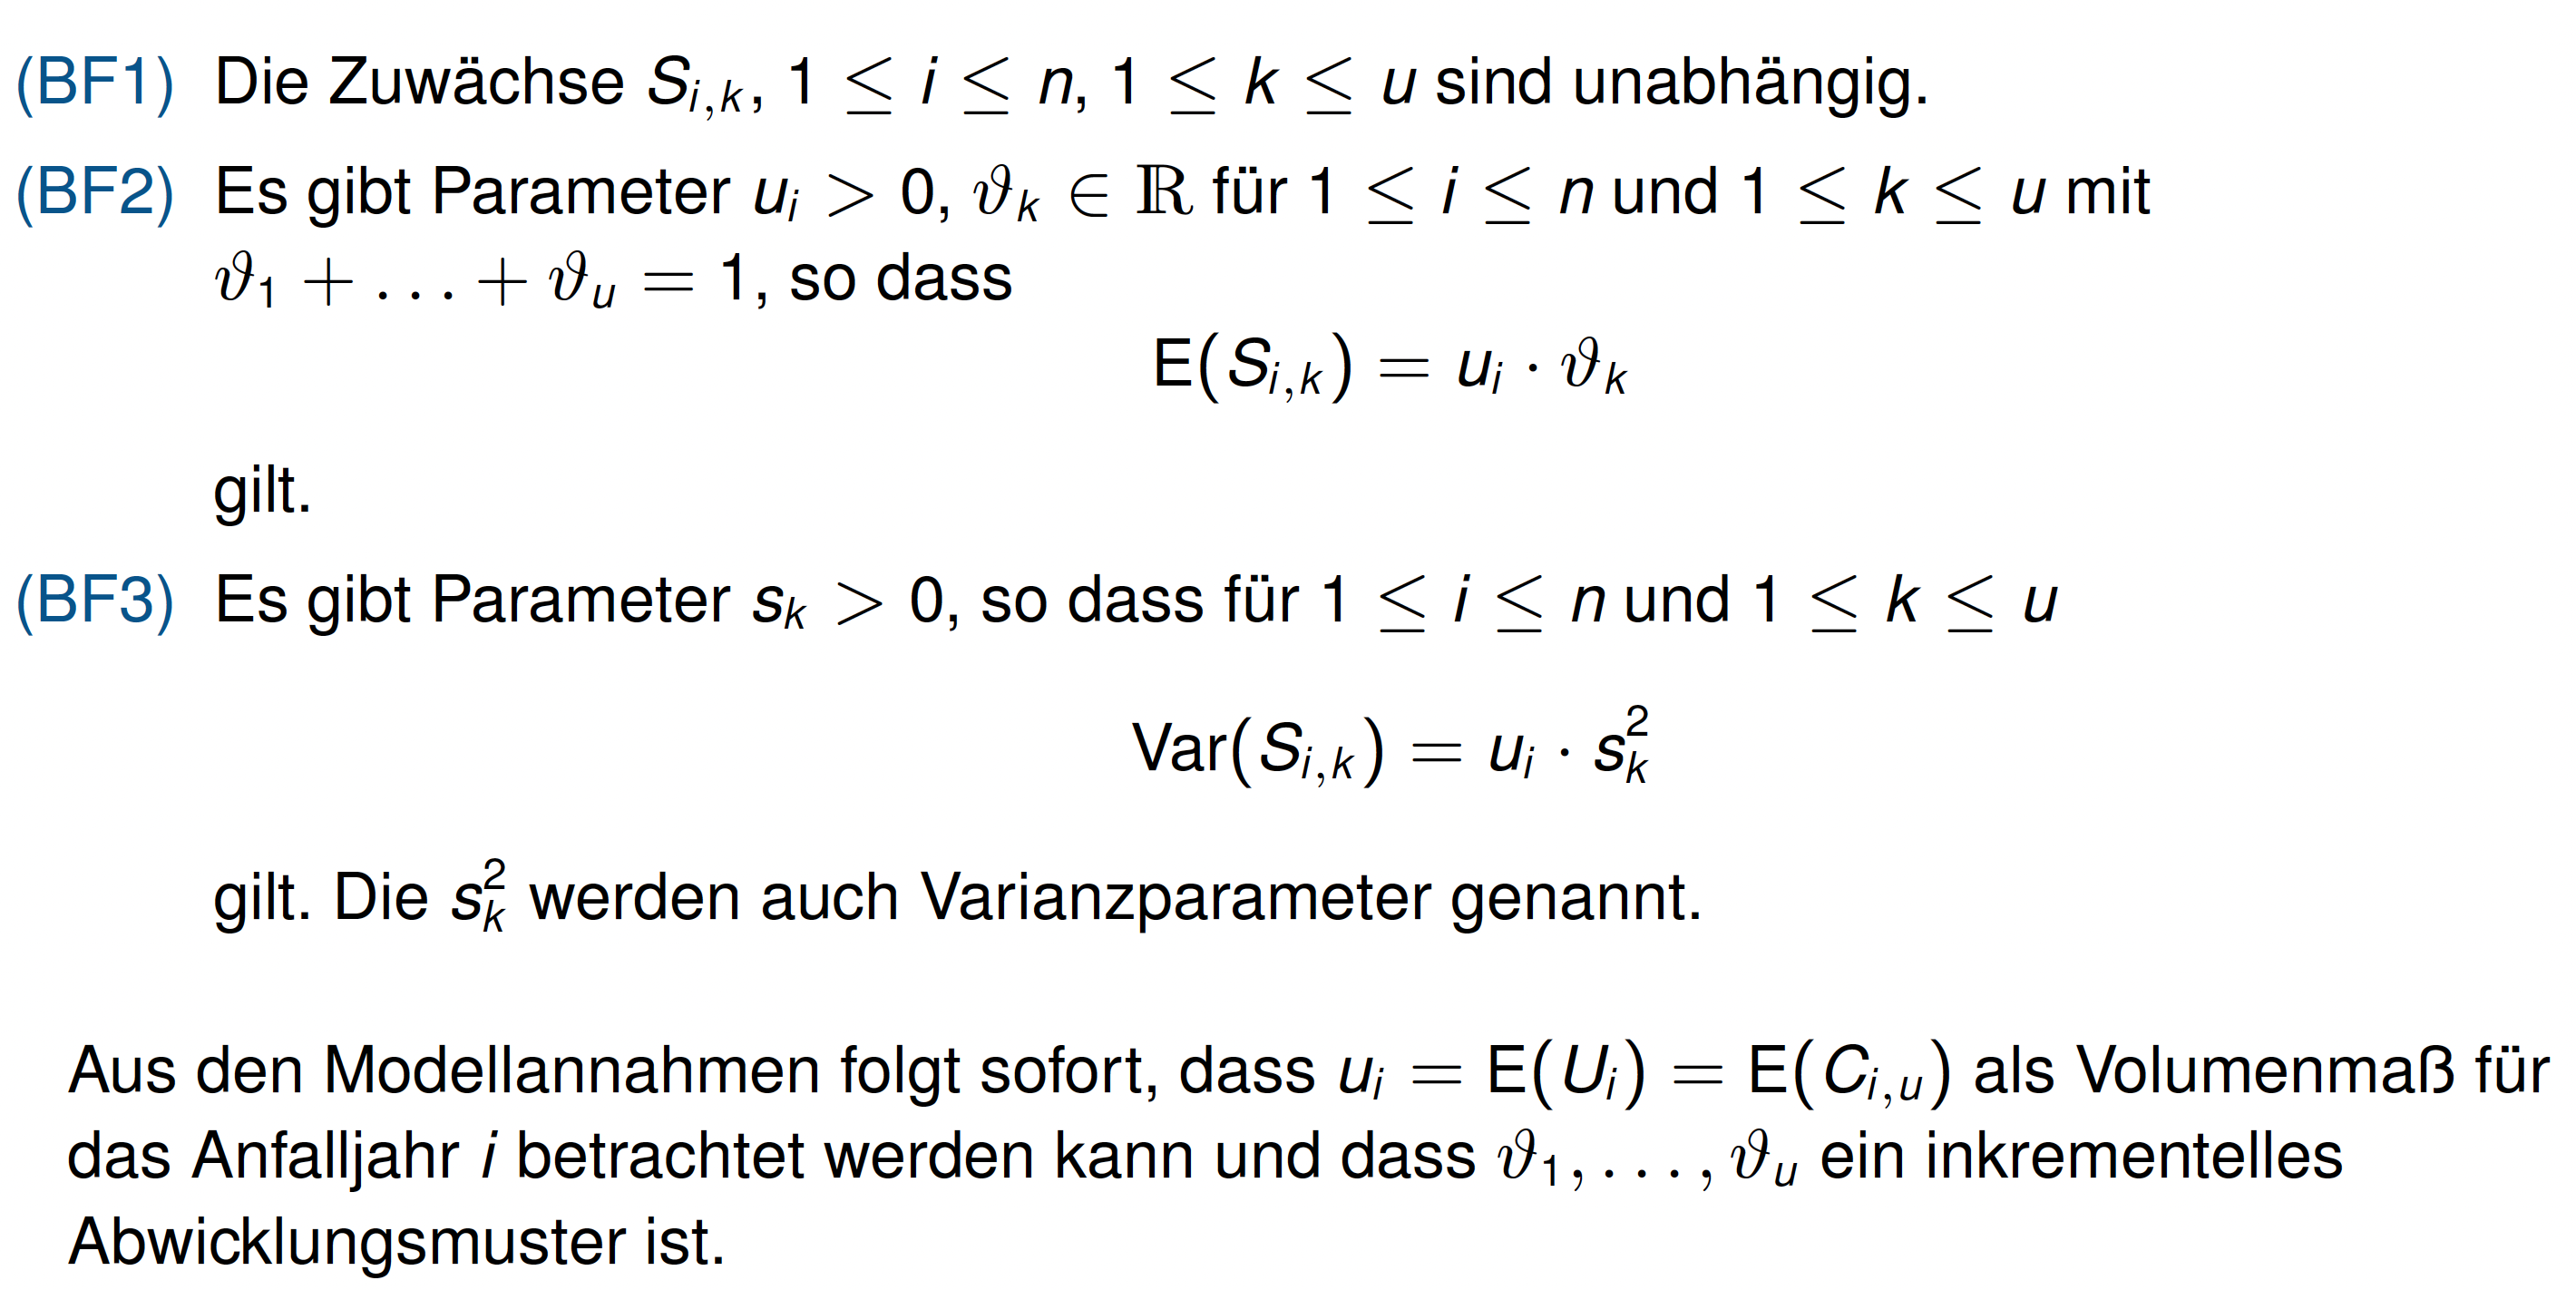
\includegraphics[width=\textwidth]{Bilder/BF3.png}
\end{figure}







































\end{document}
